% Options for packages loaded elsewhere
\PassOptionsToPackage{unicode}{hyperref}
\PassOptionsToPackage{hyphens}{url}
%
\documentclass[
]{article}
\usepackage{amsmath,amssymb}
\usepackage{iftex}
\ifPDFTeX
  \usepackage[T1]{fontenc}
  \usepackage[utf8]{inputenc}
  \usepackage{textcomp} % provide euro and other symbols
\else % if luatex or xetex
  \usepackage{unicode-math} % this also loads fontspec
  \defaultfontfeatures{Scale=MatchLowercase}
  \defaultfontfeatures[\rmfamily]{Ligatures=TeX,Scale=1}
\fi
\usepackage{lmodern}
\ifPDFTeX\else
  % xetex/luatex font selection
\fi
% Use upquote if available, for straight quotes in verbatim environments
\IfFileExists{upquote.sty}{\usepackage{upquote}}{}
\IfFileExists{microtype.sty}{% use microtype if available
  \usepackage[]{microtype}
  \UseMicrotypeSet[protrusion]{basicmath} % disable protrusion for tt fonts
}{}
\makeatletter
\@ifundefined{KOMAClassName}{% if non-KOMA class
  \IfFileExists{parskip.sty}{%
    \usepackage{parskip}
  }{% else
    \setlength{\parindent}{0pt}
    \setlength{\parskip}{6pt plus 2pt minus 1pt}}
}{% if KOMA class
  \KOMAoptions{parskip=half}}
\makeatother
\usepackage{xcolor}
\usepackage[margin=1in]{geometry}
\usepackage{color}
\usepackage{fancyvrb}
\newcommand{\VerbBar}{|}
\newcommand{\VERB}{\Verb[commandchars=\\\{\}]}
\DefineVerbatimEnvironment{Highlighting}{Verbatim}{commandchars=\\\{\}}
% Add ',fontsize=\small' for more characters per line
\usepackage{framed}
\definecolor{shadecolor}{RGB}{248,248,248}
\newenvironment{Shaded}{\begin{snugshade}}{\end{snugshade}}
\newcommand{\AlertTok}[1]{\textcolor[rgb]{0.94,0.16,0.16}{#1}}
\newcommand{\AnnotationTok}[1]{\textcolor[rgb]{0.56,0.35,0.01}{\textbf{\textit{#1}}}}
\newcommand{\AttributeTok}[1]{\textcolor[rgb]{0.13,0.29,0.53}{#1}}
\newcommand{\BaseNTok}[1]{\textcolor[rgb]{0.00,0.00,0.81}{#1}}
\newcommand{\BuiltInTok}[1]{#1}
\newcommand{\CharTok}[1]{\textcolor[rgb]{0.31,0.60,0.02}{#1}}
\newcommand{\CommentTok}[1]{\textcolor[rgb]{0.56,0.35,0.01}{\textit{#1}}}
\newcommand{\CommentVarTok}[1]{\textcolor[rgb]{0.56,0.35,0.01}{\textbf{\textit{#1}}}}
\newcommand{\ConstantTok}[1]{\textcolor[rgb]{0.56,0.35,0.01}{#1}}
\newcommand{\ControlFlowTok}[1]{\textcolor[rgb]{0.13,0.29,0.53}{\textbf{#1}}}
\newcommand{\DataTypeTok}[1]{\textcolor[rgb]{0.13,0.29,0.53}{#1}}
\newcommand{\DecValTok}[1]{\textcolor[rgb]{0.00,0.00,0.81}{#1}}
\newcommand{\DocumentationTok}[1]{\textcolor[rgb]{0.56,0.35,0.01}{\textbf{\textit{#1}}}}
\newcommand{\ErrorTok}[1]{\textcolor[rgb]{0.64,0.00,0.00}{\textbf{#1}}}
\newcommand{\ExtensionTok}[1]{#1}
\newcommand{\FloatTok}[1]{\textcolor[rgb]{0.00,0.00,0.81}{#1}}
\newcommand{\FunctionTok}[1]{\textcolor[rgb]{0.13,0.29,0.53}{\textbf{#1}}}
\newcommand{\ImportTok}[1]{#1}
\newcommand{\InformationTok}[1]{\textcolor[rgb]{0.56,0.35,0.01}{\textbf{\textit{#1}}}}
\newcommand{\KeywordTok}[1]{\textcolor[rgb]{0.13,0.29,0.53}{\textbf{#1}}}
\newcommand{\NormalTok}[1]{#1}
\newcommand{\OperatorTok}[1]{\textcolor[rgb]{0.81,0.36,0.00}{\textbf{#1}}}
\newcommand{\OtherTok}[1]{\textcolor[rgb]{0.56,0.35,0.01}{#1}}
\newcommand{\PreprocessorTok}[1]{\textcolor[rgb]{0.56,0.35,0.01}{\textit{#1}}}
\newcommand{\RegionMarkerTok}[1]{#1}
\newcommand{\SpecialCharTok}[1]{\textcolor[rgb]{0.81,0.36,0.00}{\textbf{#1}}}
\newcommand{\SpecialStringTok}[1]{\textcolor[rgb]{0.31,0.60,0.02}{#1}}
\newcommand{\StringTok}[1]{\textcolor[rgb]{0.31,0.60,0.02}{#1}}
\newcommand{\VariableTok}[1]{\textcolor[rgb]{0.00,0.00,0.00}{#1}}
\newcommand{\VerbatimStringTok}[1]{\textcolor[rgb]{0.31,0.60,0.02}{#1}}
\newcommand{\WarningTok}[1]{\textcolor[rgb]{0.56,0.35,0.01}{\textbf{\textit{#1}}}}
\usepackage{graphicx}
\makeatletter
\def\maxwidth{\ifdim\Gin@nat@width>\linewidth\linewidth\else\Gin@nat@width\fi}
\def\maxheight{\ifdim\Gin@nat@height>\textheight\textheight\else\Gin@nat@height\fi}
\makeatother
% Scale images if necessary, so that they will not overflow the page
% margins by default, and it is still possible to overwrite the defaults
% using explicit options in \includegraphics[width, height, ...]{}
\setkeys{Gin}{width=\maxwidth,height=\maxheight,keepaspectratio}
% Set default figure placement to htbp
\makeatletter
\def\fps@figure{htbp}
\makeatother
\setlength{\emergencystretch}{3em} % prevent overfull lines
\providecommand{\tightlist}{%
  \setlength{\itemsep}{0pt}\setlength{\parskip}{0pt}}
\setcounter{secnumdepth}{-\maxdimen} % remove section numbering
\ifLuaTeX
  \usepackage{selnolig}  % disable illegal ligatures
\fi
\usepackage{bookmark}
\IfFileExists{xurl.sty}{\usepackage{xurl}}{} % add URL line breaks if available
\urlstyle{same}
\hypersetup{
  pdftitle={Final\_Project},
  pdfauthor={Pankaj Gaonkar},
  hidelinks,
  pdfcreator={LaTeX via pandoc}}

\title{Final\_Project}
\author{Pankaj Gaonkar}
\date{2025-04-10}

\begin{document}
\maketitle

{
\setcounter{tocdepth}{2}
\tableofcontents
}
\section{\texorpdfstring{\textbf{ABOUT}}{ABOUT}}\label{about}

This script is designed for the analysis of the Shotgun\_POULTRY
microbiome data This script contains the statistical analysis,
exploratory plots and publication plots. Each step of the analysis is
discussed at my best capabilities.For more detailed understanding please
refer the Readme file.

\subsection{Readme file link}\label{readme-file-link}

\href{https://github.com/ppg0001/PLPA_Assignment/blob/main/README.md}{Click
Here: Readme File}

\emph{NOTE: This document is for class purpose and is intended to be
updated}

\section{\texorpdfstring{\textbf{Getting
ready}}{Getting ready}}\label{getting-ready}

\subsection{Loading packages}\label{loading-packages}

\begin{Shaded}
\begin{Highlighting}[]
\CommentTok{\# Loading Packages}
\CommentTok{\# Note: Uncomment and install/load the packages if required}

\CommentTok{\# if(!requireNamespace("BiocManager"))\{}
\CommentTok{\#   install.packages("BiocManager")}
\CommentTok{\# \}}
\CommentTok{\# BiocManager::install("phyloseq")}
\CommentTok{\# BiocManager::install("microViz")}
\CommentTok{\# BiocManager::install("microbiomeMarker")}
\CommentTok{\# }
\CommentTok{\# install.packages("remotes")}
\CommentTok{\# remotes::install\_github("david{-}barnett/microViz")}
\CommentTok{\# library(microViz)}
\CommentTok{\# }
\CommentTok{\# \#Install pairwiseAdonis package if not already installed}
\CommentTok{\# if (!requireNamespace("devtools", quietly = TRUE)) \{}
\CommentTok{\#   install.packages("devtools")}
\CommentTok{\# \}}
\CommentTok{\# devtools::install\_github("pmartinezarbizu/pairwiseAdonis/pairwiseAdonis")}

\CommentTok{\# Load the package}
\CommentTok{\# library(pairwiseAdonis)}


\FunctionTok{library}\NormalTok{(ggplot2)}
\end{Highlighting}
\end{Shaded}

\begin{verbatim}
## Warning: package 'ggplot2' was built under R version 4.4.3
\end{verbatim}

\begin{Shaded}
\begin{Highlighting}[]
\FunctionTok{library}\NormalTok{(svglite)}
\FunctionTok{library}\NormalTok{(scales)}
\FunctionTok{library}\NormalTok{(tibble)}
\FunctionTok{library}\NormalTok{(reshape2)}
\FunctionTok{library}\NormalTok{(Polychrome)}
\FunctionTok{library}\NormalTok{(RColorBrewer)}
\FunctionTok{library}\NormalTok{(readxl)}
\end{Highlighting}
\end{Shaded}

\begin{verbatim}
## Warning: package 'readxl' was built under R version 4.4.3
\end{verbatim}

\begin{Shaded}
\begin{Highlighting}[]
\FunctionTok{library}\NormalTok{(tidyverse)}
\end{Highlighting}
\end{Shaded}

\begin{verbatim}
## Warning: package 'purrr' was built under R version 4.4.2
\end{verbatim}

\begin{verbatim}
## Warning: package 'lubridate' was built under R version 4.4.2
\end{verbatim}

\begin{verbatim}
## -- Attaching core tidyverse packages ------------------------ tidyverse 2.0.0 --
## v dplyr     1.1.4     v readr     2.1.5
## v forcats   1.0.0     v stringr   1.5.1
## v lubridate 1.9.4     v tidyr     1.3.1
## v purrr     1.0.4     
## -- Conflicts ------------------------------------------ tidyverse_conflicts() --
## x readr::col_factor() masks scales::col_factor()
## x purrr::discard()    masks scales::discard()
## x dplyr::filter()     masks stats::filter()
## x dplyr::lag()        masks stats::lag()
## i Use the conflicted package (<http://conflicted.r-lib.org/>) to force all conflicts to become errors
\end{verbatim}

\begin{Shaded}
\begin{Highlighting}[]
\FunctionTok{library}\NormalTok{(ggpubr)}

\FunctionTok{library}\NormalTok{(phyloseq)}
\FunctionTok{library}\NormalTok{(vegan)}
\end{Highlighting}
\end{Shaded}

\begin{verbatim}
## Warning: package 'vegan' was built under R version 4.4.2
\end{verbatim}

\begin{verbatim}
## Loading required package: permute
## Loading required package: lattice
\end{verbatim}

\begin{Shaded}
\begin{Highlighting}[]
\FunctionTok{library}\NormalTok{(microViz)}
\end{Highlighting}
\end{Shaded}

\begin{verbatim}
## microViz version 0.12.6 - Copyright (C) 2021-2024 David Barnett
## Attaching package: 'microViz'
## The following object is masked from 'package:ggpubr':
## 
## stat_chull
## ! Website: https://david-barnett.github.io/microViz
## v Useful?  For citation details, run: `citation("microViz")`
## x Silence? `suppressPackageStartupMessages(library(microViz))`
\end{verbatim}

\begin{Shaded}
\begin{Highlighting}[]
\FunctionTok{library}\NormalTok{(microbiomeMarker)}
\end{Highlighting}
\end{Shaded}

\begin{verbatim}
## Registered S3 method overwritten by 'gplots':
##   method         from     
##   reorder.factor DescTools
## 
## Attaching package: 'microbiomeMarker'
## 
## The following object is masked from 'package:phyloseq':
## 
##     plot_heatmap
\end{verbatim}

\begin{Shaded}
\begin{Highlighting}[]
\FunctionTok{library}\NormalTok{(dplyr)}
\FunctionTok{library}\NormalTok{(tidyr)}

\FunctionTok{library}\NormalTok{(VennDiagram)}
\end{Highlighting}
\end{Shaded}

\begin{verbatim}
## Loading required package: grid
## Loading required package: futile.logger
## 
## Attaching package: 'VennDiagram'
## 
## The following object is masked from 'package:ggpubr':
## 
##     rotate
\end{verbatim}

\begin{Shaded}
\begin{Highlighting}[]
\FunctionTok{library}\NormalTok{(grid)}
\end{Highlighting}
\end{Shaded}

\subsection{Loading required input
files}\label{loading-required-input-files}

\begin{Shaded}
\begin{Highlighting}[]
\CommentTok{\# Load the microbiome realtive abundance data, sample metadata, taxanomy metadata.}
\CommentTok{\# Note: All files are present in project folder and can be uploaded relatively.}

\NormalTok{tbl\_otu }\OtherTok{\textless{}{-}} \FunctionTok{read.delim}\NormalTok{(}\StringTok{"Microbiome\_RelAb.tsv"}\NormalTok{) }\SpecialCharTok{\%\textgreater{}\%}
  \FunctionTok{column\_to\_rownames}\NormalTok{(}\AttributeTok{var =} \StringTok{"Taxon"}\NormalTok{)}

\NormalTok{mt\_smpl }\OtherTok{\textless{}{-}} \FunctionTok{read.delim}\NormalTok{(}\StringTok{"Sample\_metadata.tsv"}\NormalTok{, }
                      \CommentTok{\#row.names=1, }
                      \AttributeTok{stringsAsFactors=}\ConstantTok{TRUE}\NormalTok{) }\SpecialCharTok{\%\textgreater{}\%}
           \CommentTok{\#Duplicating sample column for rowname}
           \FunctionTok{mutate}\NormalTok{(}\AttributeTok{sample =}\NormalTok{ Sample) }\SpecialCharTok{\%\textgreater{}\%}
           \FunctionTok{column\_to\_rownames}\NormalTok{(}\AttributeTok{var =} \StringTok{"sample"}\NormalTok{)}

\CommentTok{\# Reordering factors}
\CommentTok{\# We have two fain groups: Farm types and Sample types. Within main group we have respective subgroups.}

\NormalTok{mt\_smpl}\SpecialCharTok{$}\NormalTok{Farm\_type }\OtherTok{\textless{}{-}} \FunctionTok{factor}\NormalTok{(mt\_smpl}\SpecialCharTok{$}\NormalTok{Farm\_type,}
                         \AttributeTok{levels =} \FunctionTok{c}\NormalTok{(}\StringTok{"Pullet"}\NormalTok{, }\StringTok{"Breeder"}\NormalTok{, }\StringTok{"Broiler"}\NormalTok{, }\StringTok{"Processing\_plant"}\NormalTok{)}
\NormalTok{                         )}
\NormalTok{mt\_smpl}\SpecialCharTok{$}\NormalTok{Sample\_type }\OtherTok{\textless{}{-}} \FunctionTok{factor}\NormalTok{(mt\_smpl}\SpecialCharTok{$}\NormalTok{Sample\_type,}
                             \AttributeTok{levels =} \FunctionTok{c}\NormalTok{(}\StringTok{"Litter"}\NormalTok{, }\StringTok{"Soil"}\NormalTok{)}
\NormalTok{                             )}
\CommentTok{\#unique command helps to avoid duplicates, arrange levels as per biological relevance, here based on poultry company and poultry production chain}

\NormalTok{mt\_smpl}\SpecialCharTok{$}\NormalTok{Sample\_group }\OtherTok{\textless{}{-}} \FunctionTok{factor}\NormalTok{(mt\_smpl}\SpecialCharTok{$}\NormalTok{Sample\_group, }
                               \AttributeTok{levels =} \FunctionTok{unique}\NormalTok{(}\FunctionTok{c}\NormalTok{(}\StringTok{"C2F4L"}\NormalTok{,}\StringTok{"C2F4L"}\NormalTok{,}\StringTok{"C2F4L"}\NormalTok{,}\StringTok{"C2F1L"}\NormalTok{,}\StringTok{"C3F10L"}\NormalTok{,}\StringTok{"C3F14L"}\NormalTok{,}\StringTok{"C2F4S"}\NormalTok{,}\StringTok{"C2F4S"}\NormalTok{,}\StringTok{"C2F4S"}\NormalTok{,}\StringTok{"C2F1S"}\NormalTok{,}\StringTok{"C3F10S"}\NormalTok{,}\StringTok{"C3F14S"}\NormalTok{,}\StringTok{"C2F4F"}\NormalTok{,}\StringTok{"C2F4F"}\NormalTok{,}\StringTok{"C2F4F"}\NormalTok{,}\StringTok{"C4F17L"}\NormalTok{,}\StringTok{"C4F17L"}\NormalTok{,}\StringTok{"C4F17L"}\NormalTok{,}\StringTok{"C4F8L"}\NormalTok{,}\StringTok{"C4F17S"}\NormalTok{,}\StringTok{"C4F17S"}\NormalTok{,}\StringTok{"C4F17S"}\NormalTok{,}\StringTok{"C4F8S"}\NormalTok{,}\StringTok{"C4F17F"}\NormalTok{,}\StringTok{"C4F17F"}\NormalTok{,}\StringTok{"C4F17F"}\NormalTok{,}\StringTok{"C8F40L"}\NormalTok{,}\StringTok{"C8F40L"}\NormalTok{,}\StringTok{"C8F40L"}\NormalTok{,}\StringTok{"C6F35L"}\NormalTok{,}\StringTok{"C6F37L"}\NormalTok{,}\StringTok{"C6F60L"}\NormalTok{,}\StringTok{"C7F14L"}\NormalTok{,}\StringTok{"C7F22L"}\NormalTok{,}\StringTok{"C7F81L"}\NormalTok{,}\StringTok{"C8F40S"}\NormalTok{,}\StringTok{"C8F40S"}\NormalTok{,}\StringTok{"C8F40S"}\NormalTok{,}\StringTok{"C6F35S"}\NormalTok{,}\StringTok{"C6F37S"}\NormalTok{,}\StringTok{"C6F60S"}\NormalTok{,}\StringTok{"C7F14S"}\NormalTok{,}\StringTok{"C7F22S"}\NormalTok{,}\StringTok{"C7F81S"}\NormalTok{,}\StringTok{"C8F40F"}\NormalTok{,}\StringTok{"C8F40F"}\NormalTok{,}\StringTok{"C8F40F"}\NormalTok{,}\StringTok{"C4F8PP"}\NormalTok{,}\StringTok{"C4F8PC"}\NormalTok{,}\StringTok{"C12FCHL"}\NormalTok{,}\StringTok{"C13FJBL"}\NormalTok{,}\StringTok{"C12FCHS"}\NormalTok{,}\StringTok{"C13FJBS"}\NormalTok{,}\StringTok{"C14FJOL"}\NormalTok{,}\StringTok{"C14FJOS"}\NormalTok{,}\StringTok{"C15FNSL"}\NormalTok{,}\StringTok{"C15FTCL"}\NormalTok{,}\StringTok{"C16FHWL"}\NormalTok{,}\StringTok{"C17FHEL"}\NormalTok{,}\StringTok{"C18FCLL"}\NormalTok{,}\StringTok{"C18FHHL"}\NormalTok{,}\StringTok{"C18FTGL"}\NormalTok{,}\StringTok{"C20FJAL"}\NormalTok{,}\StringTok{"C19FTTL"}\NormalTok{,}\StringTok{"C20FPHL"}\NormalTok{,}\StringTok{"C15FNSS"}\NormalTok{,}\StringTok{"C15FTCS"}\NormalTok{,}\StringTok{"C16FHWS"}\NormalTok{,}\StringTok{"C17FHES"}\NormalTok{,}\StringTok{"C18FCLS"}\NormalTok{,}\StringTok{"C18FHHS"}\NormalTok{,}\StringTok{"C18FTGS"}\NormalTok{,}\StringTok{"C20FJAS"}\NormalTok{,}\StringTok{"C19FTTS"}\NormalTok{,}\StringTok{"C20PHS"}\NormalTok{)))}


\NormalTok{mt\_smpl}\SpecialCharTok{$}\NormalTok{Sample }\OtherTok{\textless{}{-}} \FunctionTok{factor}\NormalTok{(mt\_smpl}\SpecialCharTok{$}\NormalTok{Sample, }
                               \AttributeTok{levels =} \FunctionTok{c}\NormalTok{(}\StringTok{"C2F4L1"}\NormalTok{,}\StringTok{"C2F4L2"}\NormalTok{,}\StringTok{"C2F4L3"}\NormalTok{,}\StringTok{"C2F1L"}\NormalTok{,}\StringTok{"C3F10L"}\NormalTok{,}\StringTok{"C3F14L"}\NormalTok{,}\StringTok{"C2F4S1"}\NormalTok{,}\StringTok{"C2F4S2"}\NormalTok{,}\StringTok{"C2F4S3"}\NormalTok{,}\StringTok{"C2F1S"}\NormalTok{,}\StringTok{"C3F10S"}\NormalTok{,}\StringTok{"C3F14S"}\NormalTok{,}\StringTok{"C2F4F1"}\NormalTok{,}\StringTok{"C2F4F2"}\NormalTok{,}\StringTok{"C2F4F3"}\NormalTok{,}\StringTok{"C4F17L1"}\NormalTok{,}\StringTok{"C4F17L2"}\NormalTok{,}\StringTok{"C4F17L3"}\NormalTok{,}\StringTok{"C4F8L"}\NormalTok{,}\StringTok{"C4F17S1"}\NormalTok{,}\StringTok{"C4F17S2"}\NormalTok{,}\StringTok{"C4F17S3"}\NormalTok{,}\StringTok{"C4F8S"}\NormalTok{,}\StringTok{"C4F17F1"}\NormalTok{,}\StringTok{"C4F17F2"}\NormalTok{,}\StringTok{"C4F17F3"}\NormalTok{,}\StringTok{"C8F40L1"}\NormalTok{,}\StringTok{"C8F40L2"}\NormalTok{,}\StringTok{"C8F40L3"}\NormalTok{,}\StringTok{"C6F35L"}\NormalTok{,}\StringTok{"C6F37L"}\NormalTok{,}\StringTok{"C6F60L"}\NormalTok{,}\StringTok{"C7F14L"}\NormalTok{,}\StringTok{"C7F22L"}\NormalTok{,}\StringTok{"C7F81L"}\NormalTok{,}\StringTok{"C8F40S1"}\NormalTok{,}\StringTok{"C8F40S2"}\NormalTok{,}\StringTok{"C8F40S3"}\NormalTok{,}\StringTok{"C6F35S"}\NormalTok{,}\StringTok{"C6F37S"}\NormalTok{,}\StringTok{"C6F60S"}\NormalTok{,}\StringTok{"C7F14S"}\NormalTok{,}\StringTok{"C7F22S"}\NormalTok{,}\StringTok{"C7F81S"}\NormalTok{,}\StringTok{"C8F40F1"}\NormalTok{,}\StringTok{"C8F40F2"}\NormalTok{,}\StringTok{"C8F40F3"}\NormalTok{,}\StringTok{"C4F8PP"}\NormalTok{,}\StringTok{"C4F8PC"}\NormalTok{,}\StringTok{"C12FCHL"}\NormalTok{,}\StringTok{"C13FJBL"}\NormalTok{,}\StringTok{"C12FCHS"}\NormalTok{,}\StringTok{"C13FJBS"}\NormalTok{,}\StringTok{"C14FJOL"}\NormalTok{,}\StringTok{"C14FJOS"}\NormalTok{,}\StringTok{"C15FNSL"}\NormalTok{,}\StringTok{"C15FTCL"}\NormalTok{,}\StringTok{"C16FHWL"}\NormalTok{,}\StringTok{"C17FHEL"}\NormalTok{,}\StringTok{"C18FCLL"}\NormalTok{,}\StringTok{"C18FHHL"}\NormalTok{,}\StringTok{"C18FTGL"}\NormalTok{,}\StringTok{"C20FJAL"}\NormalTok{,}\StringTok{"C19FTTL"}\NormalTok{,}\StringTok{"C20FPHL"}\NormalTok{,}\StringTok{"C15FNSS"}\NormalTok{,}\StringTok{"C15FTCS"}\NormalTok{,}\StringTok{"C16FHWS"}\NormalTok{,}\StringTok{"C17FHES"}\NormalTok{,}\StringTok{"C18FCLS"}\NormalTok{,}\StringTok{"C18FHHS"}\NormalTok{,}\StringTok{"C18FTGS"}\NormalTok{,}\StringTok{"C20FJAS"}\NormalTok{,}\StringTok{"C19FTTS"}\NormalTok{,}\StringTok{"C20PHS"}\NormalTok{))}

\CommentTok{\# Loading taxonomy metadata file}

\NormalTok{mt\_tax }\OtherTok{\textless{}{-}} \FunctionTok{read.delim}\NormalTok{(}\StringTok{"Taxonomy\_metadata.tsv"}\NormalTok{, }
                     \CommentTok{\#row.names=1, }
                     \AttributeTok{stringsAsFactors=}\ConstantTok{TRUE}\NormalTok{) }\SpecialCharTok{\%\textgreater{}\%}
          \FunctionTok{column\_to\_rownames}\NormalTok{(}\AttributeTok{var =} \StringTok{"Taxon"}\NormalTok{)}
\end{Highlighting}
\end{Shaded}

\subsection{Setting colors}\label{setting-colors}

It is important to follow a consistent coloring scheme throughout the
plots and paper. The color palette for the taxa will be created using
the package ``Polychrome''.

\begin{Shaded}
\begin{Highlighting}[]
\CommentTok{\# Creating color vectors}

\CommentTok{\# Sample colors}
\NormalTok{col\_sample }\OtherTok{\textless{}{-}} \FunctionTok{c}\NormalTok{(}\StringTok{"\#D02C2C"}\NormalTok{, }\StringTok{"\#5BBCD6"}\NormalTok{, }\StringTok{"\#F2AD00"}\NormalTok{, }\StringTok{"\#F98400"}\NormalTok{,}\StringTok{"\#00A08A"}\NormalTok{)}

\CommentTok{\# Source colors}
\NormalTok{col\_farm }\OtherTok{\textless{}{-}} \FunctionTok{c}\NormalTok{(}\StringTok{"\#E0BD48"}\NormalTok{, }\StringTok{"\#319dc8"}\NormalTok{, }\StringTok{"\#735794"}\NormalTok{, }\StringTok{"darkgrey"}\NormalTok{ )}

\NormalTok{col\_phy }\OtherTok{\textless{}{-}} \FunctionTok{c}\NormalTok{ (}\StringTok{"\#0DFFCA"}\NormalTok{,}\StringTok{"\#DDE996"}\NormalTok{,}\StringTok{"\#FB6CE0"}\NormalTok{,}\StringTok{"\#71BDA3"}\NormalTok{,}\StringTok{"\#FFAE8D"}\NormalTok{,}\StringTok{"\#A90040"}\NormalTok{,}\StringTok{"\#C2C8FE"}\NormalTok{,}\StringTok{"\#72722A"}\NormalTok{,}\StringTok{"\#D1EE0D"}\NormalTok{,}\StringTok{"\#FD89BB"}\NormalTok{,}\StringTok{"\#1CFE1C"}\NormalTok{,}\StringTok{"\#FD00FB"}\NormalTok{,}\StringTok{"\#165A6A"}\NormalTok{,}\StringTok{"\#79351C"}\NormalTok{,}\StringTok{"\#9E00FF"}\NormalTok{,}\StringTok{"\#E8DAD4"}\NormalTok{,}\StringTok{"\#26FAFD"}\NormalTok{,}\StringTok{"\#FF00B1"}\NormalTok{,}\StringTok{"\#FF7E1C"}\NormalTok{,}\StringTok{"\#51B44F"}\NormalTok{,}\StringTok{"\#9B4FA7"}\NormalTok{,}\StringTok{"\#F4C538"}\NormalTok{,}\StringTok{"\#2287E2"}\NormalTok{,}\StringTok{"\#ED3B2E"}\NormalTok{,}\StringTok{"\#1C5CFD"}\NormalTok{,}\StringTok{"\#B684FF"}\NormalTok{,}\StringTok{"\#835D75"}\NormalTok{,}\StringTok{"\#535454"}\NormalTok{)}

\NormalTok{col\_tax }\OtherTok{\textless{}{-}} \FunctionTok{c}\NormalTok{(}\StringTok{"\#b2df8a"}\NormalTok{,}\StringTok{"\#f781bf"}\NormalTok{,}\StringTok{"\#a65628"}\NormalTok{,}\StringTok{"\#ffff33"}\NormalTok{,}\StringTok{"\#984ea3"}\NormalTok{,}\StringTok{"\#4daf4a"}\NormalTok{,}\StringTok{"\#ff7f00"}\NormalTok{,}\StringTok{"\#377eb8"}\NormalTok{,}\StringTok{"\#e41a1c"}\NormalTok{,}\StringTok{"\#999999"}\NormalTok{)}

\CommentTok{\# We can use the following as our coloring scheme (uncomment if needed below)}
\CommentTok{\#swatch(col\_sample)}
\CommentTok{\#swatch(col\_farm)}
\CommentTok{\#swatch(col\_tax)}
\CommentTok{\#swatch(col\_phy)}
\end{Highlighting}
\end{Shaded}

\subsection{Print dataset structure}\label{print-dataset-structure}

\begin{Shaded}
\begin{Highlighting}[]
\FunctionTok{as\_tibble}\NormalTok{(mt\_smpl)}
\end{Highlighting}
\end{Shaded}

\begin{verbatim}
## # A tibble: 75 x 7
##    Sample Farm_Num Sample_group Farm_type Sample_type Company TotalReads
##    <fct>  <fct>    <fct>        <fct>     <fct>       <fct>        <int>
##  1 C2F1L  FN1      C2F1L        Pullet    Litter      A         78823314
##  2 C2F1S  FN1      C2F1S        Pullet    Soil        A         89536814
##  3 C2F4F1 FN2      C2F4F        Pullet    <NA>        A         41022956
##  4 C2F4F2 FN2      C2F4F        Pullet    <NA>        A         37557920
##  5 C2F4F3 FN2      C2F4F        Pullet    <NA>        A         49042293
##  6 C2F4L1 FN2      C2F4L        Pullet    Litter      A         48994993
##  7 C2F4L2 FN2      C2F4L        Pullet    Litter      A         53297079
##  8 C2F4L3 FN2      C2F4L        Pullet    Litter      A         40989190
##  9 C2F4S1 FN2      C2F4S        Pullet    Soil        A         37288480
## 10 C2F4S2 FN2      C2F4S        Pullet    Soil        A         49869876
## # i 65 more rows
\end{verbatim}

\begin{Shaded}
\begin{Highlighting}[]
\CommentTok{\#Note the NA values belong to the Fecal samples and Processing plant samples, which are not included in analysis and will not be included in further analysis for this final project.}
\end{Highlighting}
\end{Shaded}

\section{\texorpdfstring{\textbf{Metaphlan and
phyloseq}}{Metaphlan and phyloseq}}\label{metaphlan-and-phyloseq}

\begin{itemize}
\item
  Metaphlan outputs a table of relative abundances. However, phyloseq
  \emph{only accepts absolute abundances for alpha-diversity analysis}.
\item
  In order to use phyloseq the relative abundance data will be coerced
  into natural counts. This will done by multiplying the relative
  abundance by the number of mapped reads/sample (included in the table
  mt\_smpl and obtained from metaphlan output), then rounding the table,
  thus creating a dummy table of natural counts. This table preserves
  the relative abundances relationships between SGBs and allows phyloseq
  to run.
\end{itemize}

\subsection{Creating natural count
table}\label{creating-natural-count-table}

\begin{Shaded}
\begin{Highlighting}[]
\CommentTok{\#Creating a vector containing the the total number of reads in the same order as the columns in tbl\_otu so they match.}

\NormalTok{nreads }\OtherTok{\textless{}{-}}\NormalTok{ mt\_smpl}\SpecialCharTok{$}\NormalTok{TotalReads}
\CommentTok{\#nreads   \#Uncomment to see output}

\CommentTok{\#Dividing all values in tbl\_otu to shrink proportions to 0{-}1}

\NormalTok{tbl\_otu }\OtherTok{\textless{}{-}}\NormalTok{ tbl\_otu[,}\DecValTok{1}\SpecialCharTok{:}\FunctionTok{ncol}\NormalTok{(tbl\_otu)]}\SpecialCharTok{/}\DecValTok{100}

\CommentTok{\#Multiplying all values (x) of column ith (i) by the ith element of the nreads vector (i\textquotesingle{}), such as i(x)*i\textquotesingle{} = estimated read count (ecount)}

\NormalTok{tbl\_otu\_ecount }\OtherTok{\textless{}{-}} \FunctionTok{as.data.frame}\NormalTok{(}\FunctionTok{t}\NormalTok{(}\FunctionTok{t}\NormalTok{(tbl\_otu)}\SpecialCharTok{*}\NormalTok{nreads)) }\SpecialCharTok{\%\textgreater{}\%}
\NormalTok{                  dplyr}\SpecialCharTok{::}\FunctionTok{mutate}\NormalTok{(}\FunctionTok{across}\NormalTok{(is.numeric, round))}
\end{Highlighting}
\end{Shaded}

\begin{verbatim}
## Warning: There was 1 warning in `dplyr::mutate()`.
## i In argument: `across(is.numeric, round)`.
## Caused by warning:
## ! Use of bare predicate functions was deprecated in tidyselect 1.1.0.
## i Please use wrap predicates in `where()` instead.
##   # Was:
##   data %>% select(is.numeric)
## 
##   # Now:
##   data %>% select(where(is.numeric))
\end{verbatim}

\begin{Shaded}
\begin{Highlighting}[]
\CommentTok{\#The table is being transposed so that every row (i) matches with the vector entry (i\textquotesingle{}), then performing the multiplication. After this the table is transposed again to original wide shape. Then the multiplied table is fed into the mutate function which goes across and rounds all of the numerical values.}
\end{Highlighting}
\end{Shaded}

\subsection{The count data is ready to be imported into
phyloseq}\label{the-count-data-is-ready-to-be-imported-into-phyloseq}

\textbf{\emph{For our analysis, we will focus only on the bacterial
community.}}

\begin{Shaded}
\begin{Highlighting}[]
\CommentTok{\#Importing files to phyloseq}

\NormalTok{OTUcount }\OtherTok{=} \FunctionTok{otu\_table}\NormalTok{(tbl\_otu\_ecount, }
                \AttributeTok{taxa\_are\_rows =} \ConstantTok{TRUE}\NormalTok{)}
      \CommentTok{\#Needs to be parsed as matrix.}
\NormalTok{TAX }\OtherTok{=} \FunctionTok{tax\_table}\NormalTok{(}\FunctionTok{as.matrix}\NormalTok{(mt\_tax)}
\NormalTok{                )}
      \CommentTok{\#Needs to be parsed as matrix.}
\NormalTok{sampledata }\OtherTok{=} \FunctionTok{sample\_data}\NormalTok{(mt\_smpl)}

\CommentTok{\#Creating phyloseq objects}
\NormalTok{phycount\_e }\OtherTok{=} \FunctionTok{phyloseq}\NormalTok{(OTUcount, TAX, sampledata)}

\CommentTok{\#Excluding Unclassified, Archaea and Dropping other groups that needs to be excluded}
\NormalTok{phycount\_e }\OtherTok{\textless{}{-}}\NormalTok{ phycount\_e }\SpecialCharTok{\%\textgreater{}\%}
  \FunctionTok{subset\_taxa}\NormalTok{(}\SpecialCharTok{!}\NormalTok{Phylum }\SpecialCharTok{==} \StringTok{"UNCLASSIFIED"}\NormalTok{) }\CommentTok{\#\%\textgreater{}\%}
\end{Highlighting}
\end{Shaded}

\subsection{Phyloseq summary}\label{phyloseq-summary}

\begin{Shaded}
\begin{Highlighting}[]
\NormalTok{phycount\_e}
\end{Highlighting}
\end{Shaded}

\begin{verbatim}
## phyloseq-class experiment-level object
## otu_table()   OTU Table:         [ 3535 taxa and 73 samples ]
## sample_data() Sample Data:       [ 73 samples by 7 sample variables ]
## tax_table()   Taxonomy Table:    [ 3535 taxa by 7 taxonomic ranks ]
\end{verbatim}

\begin{Shaded}
\begin{Highlighting}[]
\FunctionTok{print}\NormalTok{(}\StringTok{""}\NormalTok{)}
\end{Highlighting}
\end{Shaded}

\begin{verbatim}
## [1] ""
\end{verbatim}

\begin{Shaded}
\begin{Highlighting}[]
\FunctionTok{print}\NormalTok{(}\StringTok{"Unique Phyla in phycount\_e Object"}\NormalTok{)}
\end{Highlighting}
\end{Shaded}

\begin{verbatim}
## [1] "Unique Phyla in phycount_e Object"
\end{verbatim}

\begin{Shaded}
\begin{Highlighting}[]
\FunctionTok{get\_taxa\_unique}\NormalTok{(phycount\_e, }\StringTok{"Phylum"}\NormalTok{)}
\end{Highlighting}
\end{Shaded}

\begin{verbatim}
##  [1] "Firmicutes"                  "Actinobacteria"             
##  [3] "Bacteroidetes"               "Proteobacteria"             
##  [5] "Euryarchaeota"               "Cyanobacteria"              
##  [7] "Bacteria_unclassified"       "Deinococcus_Thermus"        
##  [9] "Thaumarchaeota"              "Acidobacteria"              
## [11] "Planctomycetes"              "Chloroflexi"                
## [13] "Gemmatimonadetes"            "Nitrospirae"                
## [15] "Ascomycota"                  "Verrucomicrobia"            
## [17] "Candidatus_Thermoplasmatota" "Fusobacteria"               
## [19] "Candidatus_Melainabacteria"  "Lentisphaerae"              
## [21] "Synergistetes"               "Chlamydiae"                 
## [23] "Spirochaetes"                "Rhodothermaeota"            
## [25] "Deferribacteres"             "Candidatus_Adlerbacteria"   
## [27] "Candidatus_Saccharibacteria"
\end{verbatim}

\begin{Shaded}
\begin{Highlighting}[]
\FunctionTok{print}\NormalTok{(}\StringTok{"Sample Sources in phycount\_e object"}\NormalTok{)}
\end{Highlighting}
\end{Shaded}

\begin{verbatim}
## [1] "Sample Sources in phycount_e object"
\end{verbatim}

\begin{Shaded}
\begin{Highlighting}[]
\FunctionTok{levels}\NormalTok{(}\FunctionTok{sample\_data}\NormalTok{(phycount\_e)}\SpecialCharTok{$}\NormalTok{Sample\_type)}
\end{Highlighting}
\end{Shaded}

\begin{verbatim}
## [1] "Litter" "Soil"
\end{verbatim}

\section{\texorpdfstring{\textbf{Alpha
Diversity}}{Alpha Diversity}}\label{alpha-diversity}

\subsection{Calculating alpha-diversity
indexes}\label{calculating-alpha-diversity-indexes}

\begin{Shaded}
\begin{Highlighting}[]
\NormalTok{phycount\_div }\OtherTok{\textless{}{-}} \FunctionTok{estimate\_richness}\NormalTok{(phycount\_e, }
                                     \AttributeTok{split =} \ConstantTok{TRUE}\NormalTok{, }
                                     \AttributeTok{measures =} \FunctionTok{c}\NormalTok{(}\StringTok{"Observed"}\NormalTok{, }\StringTok{"Simpson"}\NormalTok{, }\StringTok{"Shannon"}\NormalTok{) }
\NormalTok{                                     )}
\end{Highlighting}
\end{Shaded}

\begin{verbatim}
## Warning in estimate_richness(phycount_e, split = TRUE, measures = c("Observed", : The data you have provided does not have
## any singletons. This is highly suspicious. Results of richness
## estimates (for example) are probably unreliable, or wrong, if you have already
## trimmed low-abundance taxa from the data.
## 
## We recommended that you find the un-trimmed data and retry.
\end{verbatim}

\begin{Shaded}
\begin{Highlighting}[]
\CommentTok{\#Adding sample data to table}

\NormalTok{phycount\_div }\OtherTok{\textless{}{-}} \FunctionTok{left\_join}\NormalTok{(}\FunctionTok{rownames\_to\_column}\NormalTok{(phycount\_div, }\StringTok{"Sample"}\NormalTok{),}
\NormalTok{                             mt\_smpl,}
                             \AttributeTok{by =} \StringTok{"Sample"}\NormalTok{)}

\CommentTok{\#Calculating average and standard deviation}

\NormalTok{phycount\_div }\OtherTok{\textless{}{-}}\NormalTok{ phycount\_div }\SpecialCharTok{\%\textgreater{}\%}
  \FunctionTok{group\_by}\NormalTok{(Sample\_group) }\SpecialCharTok{\%\textgreater{}\%}
  \FunctionTok{mutate}\NormalTok{(}\AttributeTok{m\_Observed =} \FunctionTok{mean}\NormalTok{(Observed),}
         \AttributeTok{sd\_Observed =} \FunctionTok{sd}\NormalTok{(Observed),}
         \AttributeTok{m\_Shannon =} \FunctionTok{mean}\NormalTok{(Shannon),}
         \AttributeTok{sd\_Shannon =} \FunctionTok{sd}\NormalTok{(Shannon),}
         \AttributeTok{m\_Simpson =} \FunctionTok{mean}\NormalTok{(Simpson),}
         \AttributeTok{sd\_Simpson =} \FunctionTok{sd}\NormalTok{(Simpson)}
\NormalTok{         )}

\NormalTok{phycount\_div}
\end{Highlighting}
\end{Shaded}

\begin{verbatim}
## # A tibble: 73 x 16
## # Groups:   Sample_group [55]
##    Sample  Observed Shannon Simpson Farm_Num Sample_group Farm_type Sample_type
##    <chr>      <dbl>   <dbl>   <dbl> <fct>    <fct>        <fct>     <fct>      
##  1 C12FCHL      320    3.85   0.961 FN21     C12FCHL      Pullet    Litter     
##  2 C12FCHS      503    5.14   0.990 FN21     C12FCHS      Pullet    Soil       
##  3 C13FJBL      219    3.40   0.927 FN22     C13FJBL      Pullet    Litter     
##  4 C13FJBS      600    5.06   0.984 FN22     C13FJBS      Pullet    Soil       
##  5 C15FNSL      299    2.91   0.808 FN24     C15FNSL      Breeder   Litter     
##  6 C15FNSS      385    4.82   0.986 FN24     C15FNSS      Breeder   Soil       
##  7 C15FTCL      398    3.34   0.884 FN25     C15FTCL      Breeder   Litter     
##  8 C15FTCS      318    3.40   0.849 FN25     C15FTCS      Breeder   Soil       
##  9 C16FHWL      390    3.90   0.952 FN26     C16FHWL      Breeder   Litter     
## 10 C16FHWS      457    3.80   0.939 FN26     C16FHWS      Breeder   Soil       
## # i 63 more rows
## # i 8 more variables: Company <fct>, TotalReads <int>, m_Observed <dbl>,
## #   sd_Observed <dbl>, m_Shannon <dbl>, sd_Shannon <dbl>, m_Simpson <dbl>,
## #   sd_Simpson <dbl>
\end{verbatim}

\begin{Shaded}
\begin{Highlighting}[]
\CommentTok{\#Write the alpha diversity values for each sample and average the replicates}
\FunctionTok{write.csv}\NormalTok{(phycount\_div, }\StringTok{"Phycount\_div\_each\_sample.csv"}\NormalTok{)}


\DocumentationTok{\#\# Table for alpha diversity}

\NormalTok{Alpha\_descriptive\_stats }\OtherTok{\textless{}{-}}\NormalTok{ phycount\_div }\SpecialCharTok{\%\textgreater{}\%}
  \FunctionTok{filter}\NormalTok{(Sample\_type }\SpecialCharTok{\%in\%} \FunctionTok{c}\NormalTok{(}\StringTok{"Litter"}\NormalTok{, }\StringTok{"Soil"}\NormalTok{)) }\SpecialCharTok{\%\textgreater{}\%}
  \FunctionTok{group\_by}\NormalTok{(Farm\_type, Sample\_type) }\SpecialCharTok{\%\textgreater{}\%}
  \FunctionTok{summarise}\NormalTok{(}
         \AttributeTok{m\_Observed =} \FunctionTok{mean}\NormalTok{(Observed),}
         \AttributeTok{sd\_Observed =} \FunctionTok{sd}\NormalTok{(Observed),}
         \AttributeTok{m\_Simpson =} \FunctionTok{mean}\NormalTok{(Simpson),}
         \AttributeTok{sd\_Simpson =} \FunctionTok{sd}\NormalTok{(Simpson),     }
         \AttributeTok{m\_Shannon =} \FunctionTok{mean}\NormalTok{(Shannon),}
         \AttributeTok{sd\_Shannon =} \FunctionTok{sd}\NormalTok{(Shannon),}

\NormalTok{  ) }\SpecialCharTok{\%\textgreater{}\%}
  \FunctionTok{ungroup}\NormalTok{()}
\end{Highlighting}
\end{Shaded}

\begin{verbatim}
## `summarise()` has grouped output by 'Farm_type'. You can override using the
## `.groups` argument.
\end{verbatim}

\begin{Shaded}
\begin{Highlighting}[]
\CommentTok{\# Print the table}
\FunctionTok{print}\NormalTok{(Alpha\_descriptive\_stats)}
\end{Highlighting}
\end{Shaded}

\begin{verbatim}
## # A tibble: 6 x 8
##   Farm_type Sample_type m_Observed sd_Observed m_Simpson sd_Simpson m_Shannon
##   <fct>     <fct>            <dbl>       <dbl>     <dbl>      <dbl>     <dbl>
## 1 Pullet    Litter            140.       105.      0.892    0.0767       2.99
## 2 Pullet    Soil              340.       168.      0.979    0.00657      4.54
## 3 Breeder   Litter            244.       105.      0.896    0.0614       3.18
## 4 Breeder   Soil              328.       159.      0.947    0.0413       4.07
## 5 Broiler   Litter            240.        58.5     0.919    0.0291       3.17
## 6 Broiler   Soil              367.       176.      0.961    0.0190       4.19
## # i 1 more variable: sd_Shannon <dbl>
\end{verbatim}

\begin{Shaded}
\begin{Highlighting}[]
\FunctionTok{write.csv}\NormalTok{(Alpha\_descriptive\_stats, }\StringTok{"Alpha\_Divertsity\_descriptive\_stats.csv"}\NormalTok{)}
\end{Highlighting}
\end{Shaded}

\subsection{Alpha diversity: t-test comparision between Litter and Soil
within each farm
types}\label{alpha-diversity-t-test-comparision-between-litter-and-soil-within-each-farm-types}

\begin{Shaded}
\begin{Highlighting}[]
\CommentTok{\# Using t.test to compare between the two groups}

\DocumentationTok{\#\#Comparing Observed Richness}
\FunctionTok{print}\NormalTok{(}\StringTok{"RICHNESS PULLET"}\NormalTok{)}
\end{Highlighting}
\end{Shaded}

\begin{verbatim}
## [1] "RICHNESS PULLET"
\end{verbatim}

\begin{Shaded}
\begin{Highlighting}[]
\NormalTok{phycount\_div }\SpecialCharTok{\%\textgreater{}\%}
  \FunctionTok{filter}\NormalTok{(Sample\_type }\SpecialCharTok{\%in\%} \FunctionTok{c}\NormalTok{(}\StringTok{"Soil"}\NormalTok{, }\StringTok{"Litter"}\NormalTok{),}
\NormalTok{         Farm\_type }\SpecialCharTok{==} \StringTok{"Pullet"}\NormalTok{) }\SpecialCharTok{\%\textgreater{}\%}
  \FunctionTok{t.test}\NormalTok{(Observed }\SpecialCharTok{\textasciitilde{}}\NormalTok{ Sample\_type, }
       \AttributeTok{data =}\NormalTok{ .}
\NormalTok{       )}
\end{Highlighting}
\end{Shaded}

\begin{verbatim}
## 
##  Welch Two Sample t-test
## 
## data:  Observed by Sample_type
## t = -2.4673, df = 8.4047, p-value = 0.0375
## alternative hypothesis: true difference in means between group Litter and group Soil is not equal to 0
## 95 percent confidence interval:
##  -384.08631  -14.58035
## sample estimates:
## mean in group Litter   mean in group Soil 
##             140.3333             339.6667
\end{verbatim}

\begin{Shaded}
\begin{Highlighting}[]
\FunctionTok{print}\NormalTok{(}\StringTok{"RICHNESS BREEDER"}\NormalTok{)}
\end{Highlighting}
\end{Shaded}

\begin{verbatim}
## [1] "RICHNESS BREEDER"
\end{verbatim}

\begin{Shaded}
\begin{Highlighting}[]
\NormalTok{phycount\_div }\SpecialCharTok{\%\textgreater{}\%}
  \FunctionTok{filter}\NormalTok{(Sample\_type }\SpecialCharTok{\%in\%} \FunctionTok{c}\NormalTok{(}\StringTok{"Soil"}\NormalTok{, }\StringTok{"Litter"}\NormalTok{),}
\NormalTok{         Farm\_type }\SpecialCharTok{==} \StringTok{"Breeder"}\NormalTok{) }\SpecialCharTok{\%\textgreater{}\%}
  \FunctionTok{t.test}\NormalTok{(Observed }\SpecialCharTok{\textasciitilde{}}\NormalTok{ Sample\_type, }
       \AttributeTok{data =}\NormalTok{ .}
\NormalTok{       )}
\end{Highlighting}
\end{Shaded}

\begin{verbatim}
## 
##  Welch Two Sample t-test
## 
## data:  Observed by Sample_type
## t = -1.3218, df = 13.876, p-value = 0.2076
## alternative hypothesis: true difference in means between group Litter and group Soil is not equal to 0
## 95 percent confidence interval:
##  -221.00037   52.55593
## sample estimates:
## mean in group Litter   mean in group Soil 
##             243.5556             327.7778
\end{verbatim}

\begin{Shaded}
\begin{Highlighting}[]
\FunctionTok{print}\NormalTok{(}\StringTok{"RICHNESS BROILER"}\NormalTok{)}
\end{Highlighting}
\end{Shaded}

\begin{verbatim}
## [1] "RICHNESS BROILER"
\end{verbatim}

\begin{Shaded}
\begin{Highlighting}[]
\NormalTok{phycount\_div }\SpecialCharTok{\%\textgreater{}\%}
  \FunctionTok{filter}\NormalTok{(Sample\_type }\SpecialCharTok{\%in\%} \FunctionTok{c}\NormalTok{(}\StringTok{"Soil"}\NormalTok{, }\StringTok{"Litter"}\NormalTok{),}
\NormalTok{         Farm\_type }\SpecialCharTok{==} \StringTok{"Broiler"}\NormalTok{) }\SpecialCharTok{\%\textgreater{}\%}
  \FunctionTok{t.test}\NormalTok{(Observed }\SpecialCharTok{\textasciitilde{}}\NormalTok{ Sample\_type, }
       \AttributeTok{data =}\NormalTok{ .}
\NormalTok{       )}
\end{Highlighting}
\end{Shaded}

\begin{verbatim}
## 
##  Welch Two Sample t-test
## 
## data:  Observed by Sample_type
## t = -2.7454, df = 18.28, p-value = 0.01317
## alternative hypothesis: true difference in means between group Litter and group Soil is not equal to 0
## 95 percent confidence interval:
##  -224.30191  -29.94809
## sample estimates:
## mean in group Litter   mean in group Soil 
##              240.125              367.250
\end{verbatim}

\begin{Shaded}
\begin{Highlighting}[]
\DocumentationTok{\#\#Comparing Shannon index}
\FunctionTok{print}\NormalTok{(}\StringTok{"SHANNON PULLET"}\NormalTok{)}
\end{Highlighting}
\end{Shaded}

\begin{verbatim}
## [1] "SHANNON PULLET"
\end{verbatim}

\begin{Shaded}
\begin{Highlighting}[]
\NormalTok{phycount\_div }\SpecialCharTok{\%\textgreater{}\%}
  \FunctionTok{filter}\NormalTok{(Sample\_type }\SpecialCharTok{\%in\%} \FunctionTok{c}\NormalTok{(}\StringTok{"Soil"}\NormalTok{, }\StringTok{"Litter"}\NormalTok{),}
\NormalTok{         Farm\_type }\SpecialCharTok{==} \StringTok{"Pullet"}\NormalTok{) }\SpecialCharTok{\%\textgreater{}\%}
  \FunctionTok{t.test}\NormalTok{(Shannon }\SpecialCharTok{\textasciitilde{}}\NormalTok{ Sample\_type, }
       \AttributeTok{data =}\NormalTok{ .}
\NormalTok{       )}
\end{Highlighting}
\end{Shaded}

\begin{verbatim}
## 
##  Welch Two Sample t-test
## 
## data:  Shannon by Sample_type
## t = -5.2641, df = 9.4962, p-value = 0.0004341
## alternative hypothesis: true difference in means between group Litter and group Soil is not equal to 0
## 95 percent confidence interval:
##  -2.2161807 -0.8913371
## sample estimates:
## mean in group Litter   mean in group Soil 
##             2.986119             4.539878
\end{verbatim}

\begin{Shaded}
\begin{Highlighting}[]
\FunctionTok{print}\NormalTok{(}\StringTok{"SHANNON BREEDER"}\NormalTok{)}
\end{Highlighting}
\end{Shaded}

\begin{verbatim}
## [1] "SHANNON BREEDER"
\end{verbatim}

\begin{Shaded}
\begin{Highlighting}[]
\NormalTok{phycount\_div }\SpecialCharTok{\%\textgreater{}\%}
  \FunctionTok{filter}\NormalTok{(Sample\_type }\SpecialCharTok{\%in\%} \FunctionTok{c}\NormalTok{(}\StringTok{"Soil"}\NormalTok{, }\StringTok{"Litter"}\NormalTok{),}
\NormalTok{         Farm\_type }\SpecialCharTok{==} \StringTok{"Breeder"}\NormalTok{) }\SpecialCharTok{\%\textgreater{}\%}
  \FunctionTok{t.test}\NormalTok{(Shannon }\SpecialCharTok{\textasciitilde{}}\NormalTok{ Sample\_type, }
       \AttributeTok{data =}\NormalTok{ .}
\NormalTok{       )}
\end{Highlighting}
\end{Shaded}

\begin{verbatim}
## 
##  Welch Two Sample t-test
## 
## data:  Shannon by Sample_type
## t = -4.6001, df = 15.972, p-value = 0.000297
## alternative hypothesis: true difference in means between group Litter and group Soil is not equal to 0
## 95 percent confidence interval:
##  -1.3030532 -0.4808508
## sample estimates:
## mean in group Litter   mean in group Soil 
##             3.177859             4.069811
\end{verbatim}

\begin{Shaded}
\begin{Highlighting}[]
\FunctionTok{print}\NormalTok{(}\StringTok{"SHANNON BROILER"}\NormalTok{)}
\end{Highlighting}
\end{Shaded}

\begin{verbatim}
## [1] "SHANNON BROILER"
\end{verbatim}

\begin{Shaded}
\begin{Highlighting}[]
\NormalTok{phycount\_div }\SpecialCharTok{\%\textgreater{}\%}
  \FunctionTok{filter}\NormalTok{(Sample\_type }\SpecialCharTok{\%in\%} \FunctionTok{c}\NormalTok{(}\StringTok{"Soil"}\NormalTok{, }\StringTok{"Litter"}\NormalTok{),}
\NormalTok{         Farm\_type }\SpecialCharTok{==} \StringTok{"Broiler"}\NormalTok{) }\SpecialCharTok{\%\textgreater{}\%}
  \FunctionTok{t.test}\NormalTok{(Shannon }\SpecialCharTok{\textasciitilde{}}\NormalTok{ Sample\_type, }
       \AttributeTok{data =}\NormalTok{ .}
\NormalTok{       )}
\end{Highlighting}
\end{Shaded}

\begin{verbatim}
## 
##  Welch Two Sample t-test
## 
## data:  Shannon by Sample_type
## t = -8.0914, df = 19.293, p-value = 1.268e-07
## alternative hypothesis: true difference in means between group Litter and group Soil is not equal to 0
## 95 percent confidence interval:
##  -1.2823304 -0.7556906
## sample estimates:
## mean in group Litter   mean in group Soil 
##             3.173157             4.192168
\end{verbatim}

\begin{Shaded}
\begin{Highlighting}[]
\DocumentationTok{\#\#Comparing Simpson index}
\FunctionTok{print}\NormalTok{(}\StringTok{"SIMPSON PULLET"}\NormalTok{)}
\end{Highlighting}
\end{Shaded}

\begin{verbatim}
## [1] "SIMPSON PULLET"
\end{verbatim}

\begin{Shaded}
\begin{Highlighting}[]
\NormalTok{phycount\_div }\SpecialCharTok{\%\textgreater{}\%}
  \FunctionTok{filter}\NormalTok{(Sample\_type }\SpecialCharTok{\%in\%} \FunctionTok{c}\NormalTok{(}\StringTok{"Soil"}\NormalTok{, }\StringTok{"Litter"}\NormalTok{),}
\NormalTok{         Farm\_type }\SpecialCharTok{==} \StringTok{"Pullet"}\NormalTok{) }\SpecialCharTok{\%\textgreater{}\%}
  \FunctionTok{t.test}\NormalTok{(Simpson }\SpecialCharTok{\textasciitilde{}}\NormalTok{ Sample\_type, }
       \AttributeTok{data =}\NormalTok{ .}
\NormalTok{       )}
\end{Highlighting}
\end{Shaded}

\begin{verbatim}
## 
##  Welch Two Sample t-test
## 
## data:  Simpson by Sample_type
## t = -2.7854, df = 5.0735, p-value = 0.03804
## alternative hypothesis: true difference in means between group Litter and group Soil is not equal to 0
## 95 percent confidence interval:
##  -0.167894531 -0.007098203
## sample estimates:
## mean in group Litter   mean in group Soil 
##            0.8919210            0.9794174
\end{verbatim}

\begin{Shaded}
\begin{Highlighting}[]
\FunctionTok{print}\NormalTok{(}\StringTok{"SIMPSON BREEDER"}\NormalTok{)}
\end{Highlighting}
\end{Shaded}

\begin{verbatim}
## [1] "SIMPSON BREEDER"
\end{verbatim}

\begin{Shaded}
\begin{Highlighting}[]
\NormalTok{phycount\_div }\SpecialCharTok{\%\textgreater{}\%}
  \FunctionTok{filter}\NormalTok{(Sample\_type }\SpecialCharTok{\%in\%} \FunctionTok{c}\NormalTok{(}\StringTok{"Soil"}\NormalTok{, }\StringTok{"Litter"}\NormalTok{),}
\NormalTok{         Farm\_type }\SpecialCharTok{==} \StringTok{"Breeder"}\NormalTok{) }\SpecialCharTok{\%\textgreater{}\%}
  \FunctionTok{t.test}\NormalTok{(Simpson }\SpecialCharTok{\textasciitilde{}}\NormalTok{ Sample\_type, }
       \AttributeTok{data =}\NormalTok{ .}
\NormalTok{       )}
\end{Highlighting}
\end{Shaded}

\begin{verbatim}
## 
##  Welch Two Sample t-test
## 
## data:  Simpson by Sample_type
## t = -2.0496, df = 14.013, p-value = 0.0596
## alternative hypothesis: true difference in means between group Litter and group Soil is not equal to 0
## 95 percent confidence interval:
##  -0.103409053  0.002342238
## sample estimates:
## mean in group Litter   mean in group Soil 
##            0.8960792            0.9466126
\end{verbatim}

\begin{Shaded}
\begin{Highlighting}[]
\FunctionTok{print}\NormalTok{(}\StringTok{"SIMPSON BROILER"}\NormalTok{)}
\end{Highlighting}
\end{Shaded}

\begin{verbatim}
## [1] "SIMPSON BROILER"
\end{verbatim}

\begin{Shaded}
\begin{Highlighting}[]
\NormalTok{phycount\_div }\SpecialCharTok{\%\textgreater{}\%}
  \FunctionTok{filter}\NormalTok{(Sample\_type }\SpecialCharTok{\%in\%} \FunctionTok{c}\NormalTok{(}\StringTok{"Soil"}\NormalTok{, }\StringTok{"Litter"}\NormalTok{),}
\NormalTok{         Farm\_type }\SpecialCharTok{==} \StringTok{"Broiler"}\NormalTok{) }\SpecialCharTok{\%\textgreater{}\%}
  \FunctionTok{t.test}\NormalTok{(Observed }\SpecialCharTok{\textasciitilde{}}\NormalTok{ Sample\_type, }
       \AttributeTok{data =}\NormalTok{ .}
\NormalTok{       )}
\end{Highlighting}
\end{Shaded}

\begin{verbatim}
## 
##  Welch Two Sample t-test
## 
## data:  Observed by Sample_type
## t = -2.7454, df = 18.28, p-value = 0.01317
## alternative hypothesis: true difference in means between group Litter and group Soil is not equal to 0
## 95 percent confidence interval:
##  -224.30191  -29.94809
## sample estimates:
## mean in group Litter   mean in group Soil 
##              240.125              367.250
\end{verbatim}

Writing alpha diversity t-test to file

\begin{Shaded}
\begin{Highlighting}[]
\DocumentationTok{\#\# Sink command, it print everything between sinks()}

\FunctionTok{set.seed}\NormalTok{(}\DecValTok{43}\NormalTok{)}
\FunctionTok{sink}\NormalTok{(}\StringTok{"AlphaDiversity\_ttest.txt"}\NormalTok{)}
 
   \DocumentationTok{\#\#Comparing OBserved Richness}
   \FunctionTok{print}\NormalTok{(}\StringTok{"RICHNESS PULLET"}\NormalTok{)}
\NormalTok{   phycount\_div }\SpecialCharTok{\%\textgreater{}\%}
     \FunctionTok{filter}\NormalTok{(Sample\_type }\SpecialCharTok{\%in\%} \FunctionTok{c}\NormalTok{(}\StringTok{"Soil"}\NormalTok{, }\StringTok{"Litter"}\NormalTok{),}
\NormalTok{            Farm\_type }\SpecialCharTok{==} \StringTok{"Pullet"}\NormalTok{) }\SpecialCharTok{\%\textgreater{}\%}
     \FunctionTok{t.test}\NormalTok{(Observed }\SpecialCharTok{\textasciitilde{}}\NormalTok{ Sample\_type, }
          \AttributeTok{data =}\NormalTok{ .}
\NormalTok{          )}
   \FunctionTok{print}\NormalTok{(}\StringTok{"RICHNESS BREEDER"}\NormalTok{)}
\NormalTok{   phycount\_div }\SpecialCharTok{\%\textgreater{}\%}
     \FunctionTok{filter}\NormalTok{(Sample\_type }\SpecialCharTok{\%in\%} \FunctionTok{c}\NormalTok{(}\StringTok{"Soil"}\NormalTok{, }\StringTok{"Litter"}\NormalTok{),}
\NormalTok{            Farm\_type }\SpecialCharTok{==} \StringTok{"Breeder"}\NormalTok{) }\SpecialCharTok{\%\textgreater{}\%}
     \FunctionTok{t.test}\NormalTok{(Observed }\SpecialCharTok{\textasciitilde{}}\NormalTok{ Sample\_type, }
          \AttributeTok{data =}\NormalTok{ .}
\NormalTok{          )}
   \FunctionTok{print}\NormalTok{(}\StringTok{"RICHNESS BROILER"}\NormalTok{)}
\NormalTok{   phycount\_div }\SpecialCharTok{\%\textgreater{}\%}
     \FunctionTok{filter}\NormalTok{(Sample\_type }\SpecialCharTok{\%in\%} \FunctionTok{c}\NormalTok{(}\StringTok{"Soil"}\NormalTok{, }\StringTok{"Litter"}\NormalTok{),}
\NormalTok{            Farm\_type }\SpecialCharTok{==} \StringTok{"Broiler"}\NormalTok{) }\SpecialCharTok{\%\textgreater{}\%}
     \FunctionTok{t.test}\NormalTok{(Observed }\SpecialCharTok{\textasciitilde{}}\NormalTok{ Sample\_type, }
          \AttributeTok{data =}\NormalTok{ .}
\NormalTok{          )}
   
   
   \DocumentationTok{\#\#Comparing Shannon index}
   \FunctionTok{print}\NormalTok{(}\StringTok{"SHANNON PULLET"}\NormalTok{)}
\NormalTok{   phycount\_div }\SpecialCharTok{\%\textgreater{}\%}
     \FunctionTok{filter}\NormalTok{(Sample\_type }\SpecialCharTok{\%in\%} \FunctionTok{c}\NormalTok{(}\StringTok{"Soil"}\NormalTok{, }\StringTok{"Litter"}\NormalTok{),}
\NormalTok{            Farm\_type }\SpecialCharTok{==} \StringTok{"Pullet"}\NormalTok{) }\SpecialCharTok{\%\textgreater{}\%}
     \FunctionTok{t.test}\NormalTok{(Shannon }\SpecialCharTok{\textasciitilde{}}\NormalTok{ Sample\_type, }
          \AttributeTok{data =}\NormalTok{ .}
\NormalTok{          )}
   \FunctionTok{print}\NormalTok{(}\StringTok{"SHANNON BREEDER"}\NormalTok{)}
\NormalTok{   phycount\_div }\SpecialCharTok{\%\textgreater{}\%}
     \FunctionTok{filter}\NormalTok{(Sample\_type }\SpecialCharTok{\%in\%} \FunctionTok{c}\NormalTok{(}\StringTok{"Soil"}\NormalTok{, }\StringTok{"Litter"}\NormalTok{),}
\NormalTok{            Farm\_type }\SpecialCharTok{==} \StringTok{"Breeder"}\NormalTok{) }\SpecialCharTok{\%\textgreater{}\%}
    \FunctionTok{t.test}\NormalTok{(Shannon }\SpecialCharTok{\textasciitilde{}}\NormalTok{ Sample\_type,}
         \AttributeTok{data =}\NormalTok{ .}
\NormalTok{         )}
  \FunctionTok{print}\NormalTok{(}\StringTok{"SHANNON BROILER"}\NormalTok{)}
\NormalTok{  phycount\_div }\SpecialCharTok{\%\textgreater{}\%}
    \FunctionTok{filter}\NormalTok{(Sample\_type }\SpecialCharTok{\%in\%} \FunctionTok{c}\NormalTok{(}\StringTok{"Soil"}\NormalTok{, }\StringTok{"Litter"}\NormalTok{),}
\NormalTok{           Farm\_type }\SpecialCharTok{==} \StringTok{"Broiler"}\NormalTok{) }\SpecialCharTok{\%\textgreater{}\%}
    \FunctionTok{t.test}\NormalTok{(Shannon }\SpecialCharTok{\textasciitilde{}}\NormalTok{ Sample\_type,}
         \AttributeTok{data =}\NormalTok{ .}
\NormalTok{         )}

  \DocumentationTok{\#\#Comparing Simpson index}
  \FunctionTok{print}\NormalTok{(}\StringTok{"SIMPSON PULLET"}\NormalTok{)}
\NormalTok{  phycount\_div }\SpecialCharTok{\%\textgreater{}\%}
    \FunctionTok{filter}\NormalTok{(Sample\_type }\SpecialCharTok{\%in\%} \FunctionTok{c}\NormalTok{(}\StringTok{"Soil"}\NormalTok{, }\StringTok{"Litter"}\NormalTok{),}
\NormalTok{           Farm\_type }\SpecialCharTok{==} \StringTok{"Pullet"}\NormalTok{) }\SpecialCharTok{\%\textgreater{}\%}
    \FunctionTok{t.test}\NormalTok{(Simpson }\SpecialCharTok{\textasciitilde{}}\NormalTok{ Sample\_type,}
         \AttributeTok{data =}\NormalTok{ .}
\NormalTok{         )}
  \FunctionTok{print}\NormalTok{(}\StringTok{"SIMPSON BREEDER"}\NormalTok{)}
\NormalTok{  phycount\_div }\SpecialCharTok{\%\textgreater{}\%}
    \FunctionTok{filter}\NormalTok{(Sample\_type }\SpecialCharTok{\%in\%} \FunctionTok{c}\NormalTok{(}\StringTok{"Soil"}\NormalTok{, }\StringTok{"Litter"}\NormalTok{),}
\NormalTok{           Farm\_type }\SpecialCharTok{==} \StringTok{"Breeder"}\NormalTok{) }\SpecialCharTok{\%\textgreater{}\%}
    \FunctionTok{t.test}\NormalTok{(Simpson }\SpecialCharTok{\textasciitilde{}}\NormalTok{ Sample\_type,}
         \AttributeTok{data =}\NormalTok{ .}
\NormalTok{         )}
  \FunctionTok{print}\NormalTok{(}\StringTok{"SIMPSON BROILER"}\NormalTok{)}
\NormalTok{  phycount\_div }\SpecialCharTok{\%\textgreater{}\%}
    \FunctionTok{filter}\NormalTok{(Sample\_type }\SpecialCharTok{\%in\%} \FunctionTok{c}\NormalTok{(}\StringTok{"Soil"}\NormalTok{, }\StringTok{"Litter"}\NormalTok{),}
\NormalTok{           Farm\_type }\SpecialCharTok{==} \StringTok{"Broiler"}\NormalTok{) }\SpecialCharTok{\%\textgreater{}\%}
    \FunctionTok{t.test}\NormalTok{(Observed }\SpecialCharTok{\textasciitilde{}}\NormalTok{ Sample\_type,}
         \AttributeTok{data =}\NormalTok{ .}
\NormalTok{         )}

\FunctionTok{sink}\NormalTok{()}
\end{Highlighting}
\end{Shaded}

Drawing Richness and Diversity plots

\begin{Shaded}
\begin{Highlighting}[]
\CommentTok{\#Creating vector for comparing samples}
\NormalTok{ complist }\OtherTok{\textless{}{-}} \FunctionTok{list}\NormalTok{(}\FunctionTok{c}\NormalTok{(}\StringTok{"Soil"}\NormalTok{, }\StringTok{"Litter"}\NormalTok{))}

\CommentTok{\#Creating vector with new names}
\NormalTok{ Farm\_name }\OtherTok{\textless{}{-}} \FunctionTok{c}\NormalTok{(}\StringTok{"Pullet"}\NormalTok{, }\StringTok{"Breeder"}\NormalTok{, }\StringTok{"Broiler"}\NormalTok{, }\StringTok{"Processing}\SpecialCharTok{\textbackslash{}n}\StringTok{Plant"}\NormalTok{)}
\FunctionTok{names}\NormalTok{(Farm\_name) }\OtherTok{\textless{}{-}} \FunctionTok{c}\NormalTok{(}\StringTok{"Pullet"}\NormalTok{, }\StringTok{"Breeder"}\NormalTok{, }\StringTok{"Broiler"}\NormalTok{, }\StringTok{"Processing\_plant"}\NormalTok{)}

\CommentTok{\#Drawing Observed Richness plot}
\NormalTok{bp\_rc }\OtherTok{\textless{}{-}} 
\NormalTok{      phycount\_div }\SpecialCharTok{\%\textgreater{}\%}
  \CommentTok{\# filter(Sample\_type == "Litter" | Sample\_type == "Soil") \%\textgreater{}\%}
  \FunctionTok{filter}\NormalTok{(Farm\_type }\SpecialCharTok{!=} \StringTok{"Processing\_plant"} \SpecialCharTok{\&}\NormalTok{ Sample\_type }\SpecialCharTok{!=} \StringTok{"Fecal"}\NormalTok{) }\SpecialCharTok{\%\textgreater{}\%}
  \FunctionTok{ggplot}\NormalTok{(}\FunctionTok{aes}\NormalTok{(}\AttributeTok{x =}\NormalTok{ Sample\_type,}
             \AttributeTok{y =}\NormalTok{ Observed, }
             \AttributeTok{fill =}\NormalTok{ Sample\_type}
\NormalTok{             )}
\NormalTok{         ) }\SpecialCharTok{+}
  \FunctionTok{geom\_boxplot}\NormalTok{() }\SpecialCharTok{+}
  \FunctionTok{ggtitle}\NormalTok{(}\StringTok{"Observed Richness"}\NormalTok{) }\SpecialCharTok{+}
  \FunctionTok{theme\_bw}\NormalTok{() }\SpecialCharTok{+}
  \FunctionTok{theme}\NormalTok{(}\AttributeTok{axis.text =} \FunctionTok{element\_text}\NormalTok{(}\AttributeTok{size =} \DecValTok{12}\NormalTok{, }
                                 \AttributeTok{color =} \StringTok{"black"}\NormalTok{, }
                                 \AttributeTok{hjust =} \FloatTok{0.5}
\NormalTok{                                   ),}
        \AttributeTok{axis.text.x =} \FunctionTok{element\_text}\NormalTok{(}\AttributeTok{angle =} \DecValTok{45}\NormalTok{,}
                                   \AttributeTok{vjust =} \DecValTok{1}\NormalTok{,}
                                   \AttributeTok{hjust =} \DecValTok{1}\NormalTok{),}
        \AttributeTok{axis.title =} \FunctionTok{element\_blank}\NormalTok{(),}
        \AttributeTok{panel.grid.minor =} \FunctionTok{element\_blank}\NormalTok{(),}
        \AttributeTok{panel.grid.major =} \FunctionTok{element\_line}\NormalTok{(}\AttributeTok{color =} \StringTok{"azure2"}\NormalTok{),}
        \AttributeTok{plot.title =} \FunctionTok{element\_text}\NormalTok{(}\AttributeTok{size =} \DecValTok{14}\NormalTok{, }\AttributeTok{face =} \StringTok{"bold"}\NormalTok{),}
        \AttributeTok{strip.background =} \FunctionTok{element\_rect}\NormalTok{(}\AttributeTok{fill =} \StringTok{"transparent"}\NormalTok{,}
                                        \AttributeTok{color =} \StringTok{"transparent"}\NormalTok{),}
        \AttributeTok{strip.text =} \FunctionTok{element\_text}\NormalTok{(}\AttributeTok{size =} \DecValTok{12}\NormalTok{,}
                                  \AttributeTok{face =} \StringTok{"bold"}
\NormalTok{                                  )}
\NormalTok{        ) }\SpecialCharTok{+}
  \FunctionTok{stat\_compare\_means}\NormalTok{(}\AttributeTok{comparisons =}\NormalTok{ complist, }
                     \AttributeTok{method =} \StringTok{"t.test"}\NormalTok{, }
                     \AttributeTok{label =} \StringTok{"p.signif"}\NormalTok{, }
                     \AttributeTok{vjust =} \DecValTok{1}
\NormalTok{                     ) }\SpecialCharTok{+}
  \FunctionTok{scale\_fill\_manual}\NormalTok{(}\AttributeTok{values =}\NormalTok{ col\_sample) }\SpecialCharTok{+}
  \CommentTok{\#facet\_grid(Farm\_type \textasciitilde{} Company,}
   \FunctionTok{facet\_grid}\NormalTok{(Farm\_type }\SpecialCharTok{\textasciitilde{}}\NormalTok{ .,}
             \AttributeTok{labeller =} \FunctionTok{labeller}\NormalTok{(}\AttributeTok{Farm\_type =}\NormalTok{ Farm\_name),}
             \AttributeTok{scales =} \StringTok{"free"}\NormalTok{,}
            \CommentTok{\#space = "free\_x"}
\NormalTok{             )}


\CommentTok{\#Drawing Shannon diversity index plot}
\NormalTok{bp\_sn }\OtherTok{\textless{}{-}} 
\NormalTok{    phycount\_div }\SpecialCharTok{\%\textgreater{}\%}
  \CommentTok{\# filter(Sample\_type == "Litter" | Sample\_type == "Soil") \%\textgreater{}\%}
  \FunctionTok{filter}\NormalTok{(Farm\_type }\SpecialCharTok{!=} \StringTok{"Processing\_plant"} \SpecialCharTok{\&}\NormalTok{ Sample\_type }\SpecialCharTok{!=} \StringTok{"Fecal"}\NormalTok{) }\SpecialCharTok{\%\textgreater{}\%}
  \FunctionTok{ggplot}\NormalTok{(}\FunctionTok{aes}\NormalTok{(}\AttributeTok{x =}\NormalTok{ Sample\_type, }
             \AttributeTok{y =}\NormalTok{ Shannon, }
             \AttributeTok{fill =}\NormalTok{ Sample\_type}
\NormalTok{             )}
\NormalTok{         ) }\SpecialCharTok{+}
  \FunctionTok{geom\_boxplot}\NormalTok{() }\SpecialCharTok{+}
  \FunctionTok{ggtitle}\NormalTok{(}\StringTok{"Shannon Diversity Index"}\NormalTok{) }\SpecialCharTok{+}
  \FunctionTok{theme\_bw}\NormalTok{() }\SpecialCharTok{+}
  \FunctionTok{theme}\NormalTok{(}\AttributeTok{axis.text =} \FunctionTok{element\_text}\NormalTok{(}\AttributeTok{size =} \DecValTok{12}\NormalTok{, }
                                 \AttributeTok{color =} \StringTok{"black"}\NormalTok{, }
                                 \AttributeTok{hjust =} \FloatTok{0.5}
\NormalTok{                                   ),}
        \AttributeTok{axis.text.x =} \FunctionTok{element\_text}\NormalTok{(}\AttributeTok{angle =} \DecValTok{45}\NormalTok{,}
                                   \AttributeTok{vjust =} \DecValTok{1}\NormalTok{,}
                                   \AttributeTok{hjust =} \DecValTok{1}\NormalTok{),}
        \AttributeTok{axis.title =} \FunctionTok{element\_blank}\NormalTok{(),}
        \AttributeTok{panel.grid.minor =} \FunctionTok{element\_blank}\NormalTok{(),}
        \AttributeTok{panel.grid.major =} \FunctionTok{element\_line}\NormalTok{(}\AttributeTok{color =} \StringTok{"azure2"}\NormalTok{),}
        \AttributeTok{plot.title =} \FunctionTok{element\_text}\NormalTok{(}\AttributeTok{size =} \DecValTok{14}\NormalTok{, }\AttributeTok{face =} \StringTok{"bold"}\NormalTok{),}
        \AttributeTok{strip.background =} \FunctionTok{element\_rect}\NormalTok{(}\AttributeTok{fill =} \StringTok{"transparent"}\NormalTok{,}
                                        \AttributeTok{color =} \StringTok{"transparent"}\NormalTok{),}
        \AttributeTok{strip.text =} \FunctionTok{element\_text}\NormalTok{(}\AttributeTok{size =} \DecValTok{12}\NormalTok{,}
                                  \AttributeTok{face =} \StringTok{"bold"}
\NormalTok{                                  )}
\NormalTok{        ) }\SpecialCharTok{+}
  \FunctionTok{stat\_compare\_means}\NormalTok{(}\AttributeTok{comparisons =}\NormalTok{ complist, }
                     \AttributeTok{method =} \StringTok{"t.test"}\NormalTok{, }
                     \AttributeTok{label =} \StringTok{"p.signif"}\NormalTok{, }
                     \AttributeTok{vjust =} \DecValTok{1}
\NormalTok{                     ) }\SpecialCharTok{+}
  \FunctionTok{scale\_fill\_manual}\NormalTok{(}\AttributeTok{values =}\NormalTok{ col\_sample) }\SpecialCharTok{+}
  \CommentTok{\#facet\_grid(Farm\_type \textasciitilde{} Company,}
  \FunctionTok{facet\_grid}\NormalTok{(Farm\_type }\SpecialCharTok{\textasciitilde{}}\NormalTok{ .,}
             \AttributeTok{labeller =} \FunctionTok{labeller}\NormalTok{(}\AttributeTok{Farm\_type =}\NormalTok{ Farm\_name),}
             \AttributeTok{scales =} \StringTok{"free"}\NormalTok{,}
            \AttributeTok{space =} \StringTok{"free\_x"}
\NormalTok{             )}


\CommentTok{\#Drawing Simpson diversity index plot}
\NormalTok{bp\_sp }\OtherTok{\textless{}{-}} 
\NormalTok{  phycount\_div }\SpecialCharTok{\%\textgreater{}\%}
  \CommentTok{\# filter(Sample\_type == "Litter" | Sample\_type == "Soil") \%\textgreater{}\%}
  \FunctionTok{filter}\NormalTok{(Farm\_type }\SpecialCharTok{!=} \StringTok{"Processing\_plant"} \SpecialCharTok{\&}\NormalTok{ Sample\_type }\SpecialCharTok{!=} \StringTok{"Fecal"}\NormalTok{) }\SpecialCharTok{\%\textgreater{}\%}
  \FunctionTok{ggplot}\NormalTok{(}\FunctionTok{aes}\NormalTok{(}\AttributeTok{x =}\NormalTok{ Sample\_type,}
             \AttributeTok{y =}\NormalTok{ Simpson, }
             \AttributeTok{fill =}\NormalTok{ Sample\_type}
\NormalTok{                    )}
\NormalTok{                ) }\SpecialCharTok{+}
  \FunctionTok{geom\_boxplot}\NormalTok{() }\SpecialCharTok{+}
  \FunctionTok{ggtitle}\NormalTok{(}\StringTok{"Simpson Diversity Index"}\NormalTok{) }\SpecialCharTok{+}
  \FunctionTok{theme\_bw}\NormalTok{() }\SpecialCharTok{+}
  \FunctionTok{theme}\NormalTok{(}\AttributeTok{axis.text =} \FunctionTok{element\_text}\NormalTok{(}\AttributeTok{size =} \DecValTok{12}\NormalTok{, }
                                 \AttributeTok{color =} \StringTok{"black"}\NormalTok{, }
                                 \AttributeTok{hjust =} \FloatTok{0.5}
\NormalTok{                                   ),}
        \AttributeTok{axis.text.x =} \FunctionTok{element\_text}\NormalTok{(}\AttributeTok{angle =} \DecValTok{45}\NormalTok{,}
                                   \AttributeTok{vjust =} \DecValTok{1}\NormalTok{,}
                                   \AttributeTok{hjust =} \DecValTok{1}\NormalTok{),}
        \AttributeTok{axis.title =} \FunctionTok{element\_blank}\NormalTok{(),}
        \AttributeTok{panel.grid.minor =} \FunctionTok{element\_blank}\NormalTok{(),}
        \AttributeTok{panel.grid.major =} \FunctionTok{element\_line}\NormalTok{(}\AttributeTok{color =} \StringTok{"azure2"}\NormalTok{),}
        \AttributeTok{plot.title =} \FunctionTok{element\_text}\NormalTok{(}\AttributeTok{size =} \DecValTok{14}\NormalTok{, }\AttributeTok{face =} \StringTok{"bold"}\NormalTok{),}
        \AttributeTok{strip.background =} \FunctionTok{element\_rect}\NormalTok{(}\AttributeTok{fill =} \StringTok{"transparent"}\NormalTok{,}
                                        \AttributeTok{color =} \StringTok{"transparent"}\NormalTok{),}
        \AttributeTok{strip.text =} \FunctionTok{element\_text}\NormalTok{(}\AttributeTok{size =} \DecValTok{12}\NormalTok{,}
                                  \AttributeTok{face =} \StringTok{"bold"}
\NormalTok{                                  )}
\NormalTok{        ) }\SpecialCharTok{+}
  \FunctionTok{stat\_compare\_means}\NormalTok{(}\AttributeTok{comparisons =}\NormalTok{ complist, }
                     \AttributeTok{method =} \StringTok{"t.test"}\NormalTok{, }
                     \AttributeTok{label =} \StringTok{"p.signif"}\NormalTok{, }
                     \AttributeTok{vjust =} \DecValTok{1}
\NormalTok{                     ) }\SpecialCharTok{+}
  \FunctionTok{scale\_fill\_manual}\NormalTok{(}\AttributeTok{values =}\NormalTok{ col\_sample) }\SpecialCharTok{+}
  \CommentTok{\#facet\_grid(Farm\_type \textasciitilde{} Company,}
  \FunctionTok{facet\_grid}\NormalTok{(Farm\_type }\SpecialCharTok{\textasciitilde{}}\NormalTok{ .,}
             \AttributeTok{labeller =} \FunctionTok{labeller}\NormalTok{(}\AttributeTok{Farm\_type =}\NormalTok{ Farm\_name),}
             \AttributeTok{scales =} \StringTok{"free"}\NormalTok{,}
            \AttributeTok{space =} \StringTok{"free\_x"}
\NormalTok{             )}
\end{Highlighting}
\end{Shaded}

\begin{Shaded}
\begin{Highlighting}[]
\NormalTok{bp\_rc}
\end{Highlighting}
\end{Shaded}

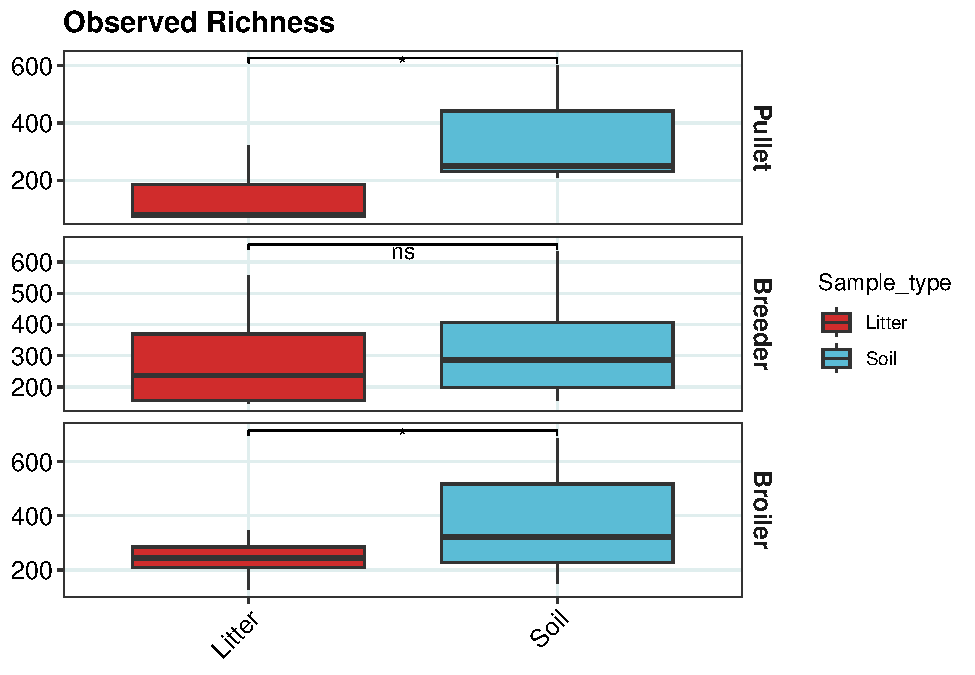
\includegraphics{Final_Project_Pankaj_files/figure-latex/drawing alpha diversity box plots-1.pdf}

\begin{Shaded}
\begin{Highlighting}[]
\NormalTok{bp\_sn}
\end{Highlighting}
\end{Shaded}

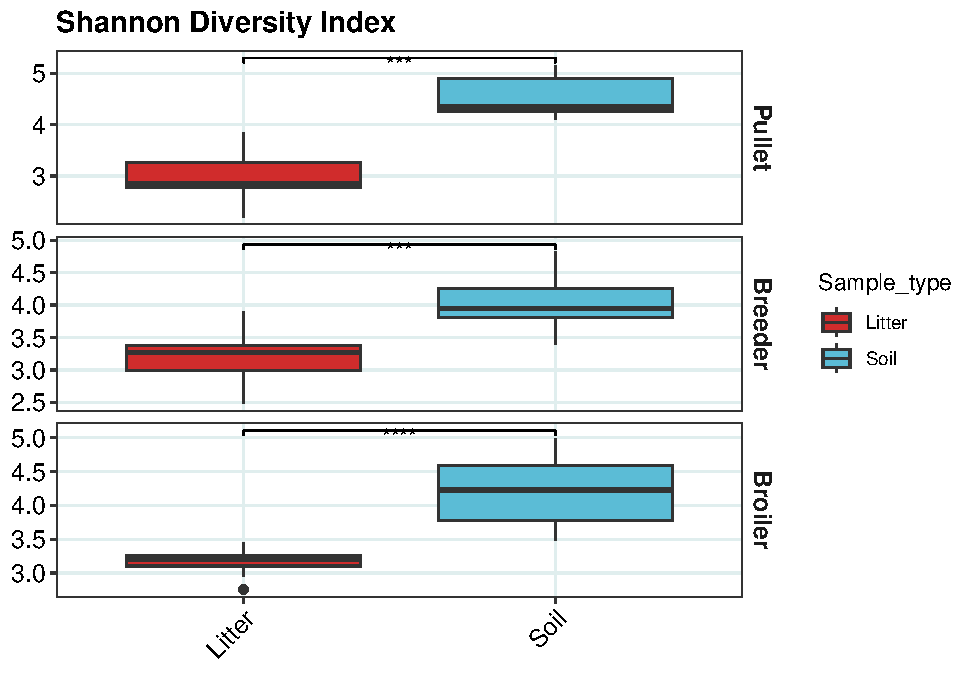
\includegraphics{Final_Project_Pankaj_files/figure-latex/drawing alpha diversity box plots-2.pdf}

\begin{Shaded}
\begin{Highlighting}[]
\NormalTok{bp\_sp}
\end{Highlighting}
\end{Shaded}

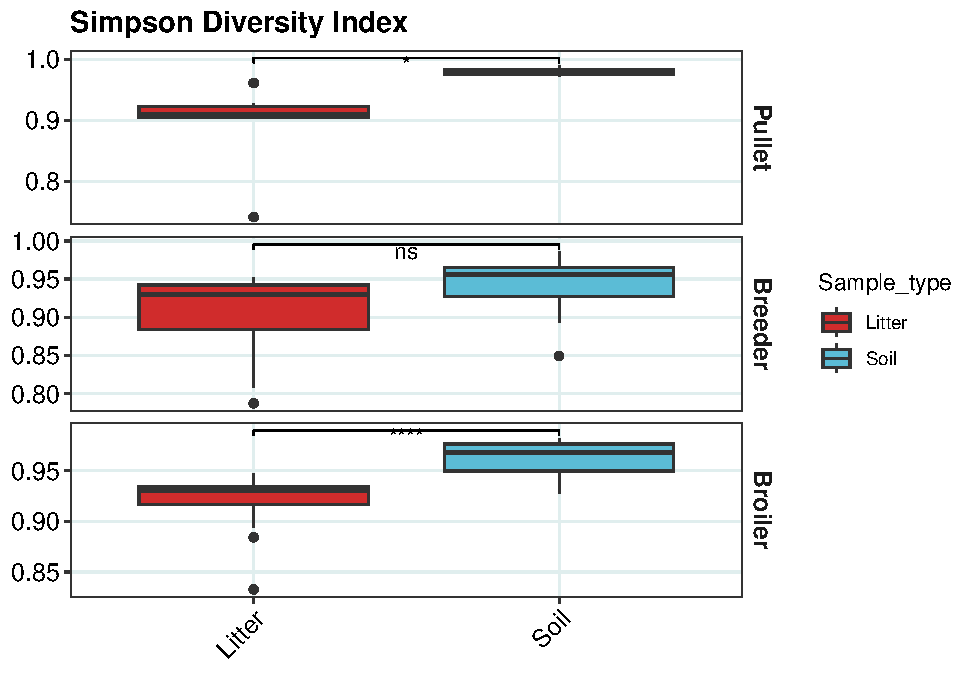
\includegraphics{Final_Project_Pankaj_files/figure-latex/drawing alpha diversity box plots-3.pdf}

Saving combined alpha diversity plots

\begin{Shaded}
\begin{Highlighting}[]
\CommentTok{\#Saving plots}

\CommentTok{\#Combined plots}
\NormalTok{combined\_plot\_Alpha\_Diversity }\OtherTok{\textless{}{-}} \FunctionTok{ggarrange}\NormalTok{(bp\_rc, bp\_sn, bp\_sp,}
                           \AttributeTok{ncol =} \DecValTok{3}\NormalTok{,}
                           \AttributeTok{nrow =} \DecValTok{1}\NormalTok{,}
                           \AttributeTok{common.legend =} \ConstantTok{TRUE}
\NormalTok{)}


\CommentTok{\#Saving plots}
\FunctionTok{ggsave}\NormalTok{(}\AttributeTok{filename =} \StringTok{"Alpha\_Diversity\_Plots.svg"}\NormalTok{,}
       \AttributeTok{plot =}\NormalTok{ combined\_plot\_Alpha\_Diversity,}
       \AttributeTok{device =} \StringTok{"svg"}\NormalTok{,}
       \AttributeTok{units =} \StringTok{"mm"}\NormalTok{,}
       \AttributeTok{width =} \DecValTok{300}\NormalTok{,}
       \AttributeTok{height =} \DecValTok{250}\NormalTok{)}
\end{Highlighting}
\end{Shaded}

\subsection{Alpha diversity result
explanation:}\label{alpha-diversity-result-explanation}

In our study, observed richness and Simpson diversity index were higher
in the soil during the pullet and broiler stages, whereas no significant
differences were found between litter and soil in the breeder stage.
Moreover, the Shannon diversity index was higher in soil samples than in
litter across all production stages. These findings indicate that soil
contains a more diverse and evenly distributed microbiome, whereas
litter is a more selective environment with limited microbes that make
up its composition.

\section{\texorpdfstring{\textbf{Exploring the microbial
community}}{Exploring the microbial community}}\label{exploring-the-microbial-community}

\subsection{Lets check which phylum are overall present in our
dataset}\label{lets-check-which-phylum-are-overall-present-in-our-dataset}

\begin{Shaded}
\begin{Highlighting}[]
\FunctionTok{table}\NormalTok{(}\FunctionTok{tax\_table}\NormalTok{(phycount\_e)[,}\StringTok{"Phylum"}\NormalTok{])}
\end{Highlighting}
\end{Shaded}

\begin{verbatim}
## 
##               Acidobacteria              Actinobacteria 
##                          10                         964 
##                  Ascomycota       Bacteria_unclassified 
##                           3                           2 
##               Bacteroidetes    Candidatus_Adlerbacteria 
##                         398                           1 
##  Candidatus_Melainabacteria Candidatus_Saccharibacteria 
##                           6                           2 
## Candidatus_Thermoplasmatota                  Chlamydiae 
##                           3                           4 
##                 Chloroflexi               Cyanobacteria 
##                           6                          54 
##             Deferribacteres         Deinococcus_Thermus 
##                           1                          21 
##               Euryarchaeota                  Firmicutes 
##                          15                         742 
##                Fusobacteria            Gemmatimonadetes 
##                           2                           2 
##               Lentisphaerae                 Nitrospirae 
##                           4                           4 
##              Planctomycetes              Proteobacteria 
##                          20                        1246 
##             Rhodothermaeota                Spirochaetes 
##                           1                           3 
##               Synergistetes              Thaumarchaeota 
##                           1                           8 
##             Verrucomicrobia 
##                          12
\end{verbatim}

\subsection{Microbial community bar
plots}\label{microbial-community-bar-plots}

First step in visualizing the community structure. In order to create
the barplots, the data needs to be transformed from wide to long. This
will also allow all the metadata to be incorporated into the table

\begin{Shaded}
\begin{Highlighting}[]
\CommentTok{\#Melting table}

\NormalTok{tbl\_mstr\_pc }\OtherTok{\textless{}{-}} \FunctionTok{melt}\NormalTok{(}\FunctionTok{rownames\_to\_column}\NormalTok{(tbl\_otu, }\AttributeTok{var =} \StringTok{"Taxon"}\NormalTok{),}
                 \AttributeTok{id.vars =} \FunctionTok{c}\NormalTok{(}\StringTok{"Taxon"}\NormalTok{),}
                 \AttributeTok{variable.name =} \StringTok{"Sample"}\NormalTok{,}
                 \AttributeTok{value.name =} \StringTok{"Count"}\NormalTok{) }\SpecialCharTok{\%\textgreater{}\%}
\CommentTok{\#Adding Metadata}
            \FunctionTok{left\_join}\NormalTok{(mt\_smpl,}
                      \AttributeTok{by =} \StringTok{"Sample"}\NormalTok{) }\SpecialCharTok{\%\textgreater{}\%}
            \FunctionTok{left\_join}\NormalTok{(}\FunctionTok{rownames\_to\_column}\NormalTok{(mt\_tax, }\AttributeTok{var =} \StringTok{"Taxon"}\NormalTok{),}
                      \AttributeTok{by =} \StringTok{"Taxon"}\NormalTok{)}
\end{Highlighting}
\end{Shaded}

Re-ordering factors so that the main colors of the swatch correspond to
the most abundant phyla across:

\begin{Shaded}
\begin{Highlighting}[]
\CommentTok{\#Summarizing counts by phyla}

\NormalTok{tbl\_mstr\_pc }\SpecialCharTok{\%\textgreater{}\%} 
  \FunctionTok{group\_by}\NormalTok{(Phylum) }\SpecialCharTok{\%\textgreater{}\%} 
  \FunctionTok{summarise}\NormalTok{(}\AttributeTok{Count =} \FunctionTok{sum}\NormalTok{(Count)) }\SpecialCharTok{\%\textgreater{}\%} 
  \FunctionTok{arrange}\NormalTok{(Count) }\SpecialCharTok{\%\textgreater{}\%}
  \FunctionTok{select}\NormalTok{(Phylum) }\SpecialCharTok{\%\textgreater{}\%}
  \FunctionTok{ungroup}\NormalTok{()}
\end{Highlighting}
\end{Shaded}

\begin{verbatim}
## # A tibble: 28 x 1
##    Phylum                     
##    <fct>                      
##  1 Deferribacteres            
##  2 Rhodothermaeota            
##  3 Candidatus_Adlerbacteria   
##  4 Candidatus_Saccharibacteria
##  5 Lentisphaerae              
##  6 Spirochaetes               
##  7 Ascomycota                 
##  8 Chlamydiae                 
##  9 Synergistetes              
## 10 Verrucomicrobia            
## # i 18 more rows
\end{verbatim}

\begin{Shaded}
\begin{Highlighting}[]
\CommentTok{\#Reordering factors in Phylum column according to most abundant.}
\CommentTok{\#NOTE: Phyla will be reordered in ascending order (from least to most). This allows us to drop some levels (ex: Unclassified), without changing the color key for the other levels}

\NormalTok{tbl\_mstr\_pc}\SpecialCharTok{$}\NormalTok{Phylum }\OtherTok{\textless{}{-}} \FunctionTok{factor}\NormalTok{(tbl\_mstr\_pc}\SpecialCharTok{$}\NormalTok{Phylum, }
                          \AttributeTok{levels =} \FunctionTok{c}\NormalTok{(}\StringTok{"Deferribacteres"}\NormalTok{,}\StringTok{"Rhodothermaeota"}\NormalTok{,}\StringTok{"Candidatus\_Adlerbacteria"}\NormalTok{,}\StringTok{"Candidatus\_Saccharibacteria"}\NormalTok{,}\StringTok{"Lentisphaerae"}\NormalTok{,}\StringTok{"Spirochaetes"}\NormalTok{,}\StringTok{"Chlamydiae"}\NormalTok{,}\StringTok{"Synergistetes"}\NormalTok{,}\StringTok{"Verrucomicrobia"}\NormalTok{,}\StringTok{"Candidatus\_Thermoplasmatota"}\NormalTok{,}\StringTok{"Gemmatimonadetes"}\NormalTok{,}\StringTok{"Nitrospirae"}\NormalTok{,}\StringTok{"Candidatus\_Melainabacteria"}\NormalTok{,}\StringTok{"Bacteria\_unclassified"}\NormalTok{,}\StringTok{"Fusobacteria"}\NormalTok{,}\StringTok{"Acidobacteria"}\NormalTok{,}\StringTok{"Planctomycetes"}\NormalTok{,}\StringTok{"Chloroflexi"}\NormalTok{,}\StringTok{"Deinococcus\_Thermus"}\NormalTok{,}\StringTok{"Cyanobacteria"}\NormalTok{,}\StringTok{"Bacteroidetes"}\NormalTok{,}\StringTok{"Proteobacteria"}\NormalTok{,}\StringTok{"Actinobacteria"}\NormalTok{,}\StringTok{"Firmicutes"}\NormalTok{,}\StringTok{"Ascomycota"}\NormalTok{,}\StringTok{"Thaumarchaeota"}\NormalTok{,}\StringTok{"Euryarchaeota"}\NormalTok{,}\StringTok{"UNCLASSIFIED"}\NormalTok{))}
\end{Highlighting}
\end{Shaded}

Creating summarised table for barplots

\begin{Shaded}
\begin{Highlighting}[]
\NormalTok{tbl\_mstr\_bp }\OtherTok{\textless{}{-}}\NormalTok{ tbl\_mstr\_pc }\SpecialCharTok{\%\textgreater{}\%}
  \FunctionTok{group\_by}\NormalTok{(Sample, Phylum) }\SpecialCharTok{\%\textgreater{}\%}
  \FunctionTok{summarise}\NormalTok{(}\AttributeTok{Count =} \FunctionTok{sum}\NormalTok{(Count)}
\NormalTok{            ) }\SpecialCharTok{\%\textgreater{}\%}
  \FunctionTok{left\_join}\NormalTok{(mt\_smpl, }\AttributeTok{by =} \StringTok{"Sample"}\NormalTok{) }\SpecialCharTok{\%\textgreater{}\%}
  \FunctionTok{distinct}\NormalTok{() }\SpecialCharTok{\%\textgreater{}\%}
  \FunctionTok{droplevels}\NormalTok{() }\SpecialCharTok{\%\textgreater{}\%}
\NormalTok{  ungroup}
\end{Highlighting}
\end{Shaded}

\begin{verbatim}
## `summarise()` has grouped output by 'Sample'. You can override using the
## `.groups` argument.
\end{verbatim}

creating averaged table

\begin{Shaded}
\begin{Highlighting}[]
\CommentTok{\# Averaging taxons by Sample\_group}

\NormalTok{tbl\_mstr\_av }\OtherTok{\textless{}{-}}\NormalTok{ tbl\_mstr\_pc }\SpecialCharTok{\%\textgreater{}\%}
  \FunctionTok{group\_by}\NormalTok{(Taxon, Sample\_group) }\SpecialCharTok{\%\textgreater{}\%}
  \FunctionTok{summarise}\NormalTok{(}\AttributeTok{Count =} \FunctionTok{mean}\NormalTok{(Count)) }\SpecialCharTok{\%\textgreater{}\%}
  \FunctionTok{left\_join}\NormalTok{(}\FunctionTok{select}\NormalTok{(mt\_smpl, }\SpecialCharTok{!}\FunctionTok{c}\NormalTok{(Sample, TotalReads)), }\AttributeTok{by =} \StringTok{"Sample\_group"}\NormalTok{) }\SpecialCharTok{\%\textgreater{}\%}
  \FunctionTok{left\_join}\NormalTok{(}\FunctionTok{rownames\_to\_column}\NormalTok{(mt\_tax, }\AttributeTok{var =} \StringTok{"Taxon"}\NormalTok{), }\AttributeTok{by =} \StringTok{"Taxon"}\NormalTok{) }\SpecialCharTok{\%\textgreater{}\%}
  \FunctionTok{distinct}\NormalTok{() }\SpecialCharTok{\%\textgreater{}\%}
  \FunctionTok{droplevels}\NormalTok{() }\SpecialCharTok{\%\textgreater{}\%}
  \FunctionTok{ungroup}\NormalTok{()}
\end{Highlighting}
\end{Shaded}

\begin{verbatim}
## `summarise()` has grouped output by 'Taxon'. You can override using the
## `.groups` argument.
\end{verbatim}

\begin{verbatim}
## Warning in left_join(., select(mt_smpl, !c(Sample, TotalReads)), by = "Sample_group"): Detected an unexpected many-to-many relationship between `x` and `y`.
## i Row 1 of `x` matches multiple rows in `y`.
## i Row 6 of `y` matches multiple rows in `x`.
## i If a many-to-many relationship is expected, set `relationship =
##   "many-to-many"` to silence this warning.
\end{verbatim}

\begin{Shaded}
\begin{Highlighting}[]
\DocumentationTok{\#\#Summarising by Phylum count}

\NormalTok{tbl\_mstr\_av\_bp }\OtherTok{\textless{}{-}}\NormalTok{ tbl\_mstr\_av }\SpecialCharTok{\%\textgreater{}\%}
  \FunctionTok{group\_by}\NormalTok{(Phylum, Sample\_group) }\SpecialCharTok{\%\textgreater{}\%}
  \FunctionTok{summarise}\NormalTok{(}\AttributeTok{Count =} \FunctionTok{sum}\NormalTok{(Count)) }\SpecialCharTok{\%\textgreater{}\%}
  \FunctionTok{left\_join}\NormalTok{(}\FunctionTok{select}\NormalTok{(mt\_smpl, }\SpecialCharTok{!}\FunctionTok{c}\NormalTok{(Sample, TotalReads)), }\AttributeTok{by =} \StringTok{"Sample\_group"}\NormalTok{) }\SpecialCharTok{\%\textgreater{}\%}
  \FunctionTok{distinct}\NormalTok{() }\SpecialCharTok{\%\textgreater{}\%}
  \FunctionTok{droplevels}\NormalTok{() }\SpecialCharTok{\%\textgreater{}\%}
  \FunctionTok{ungroup}\NormalTok{()}
\end{Highlighting}
\end{Shaded}

\begin{verbatim}
## `summarise()` has grouped output by 'Phylum'. You can override using the
## `.groups` argument.
\end{verbatim}

\begin{verbatim}
## Warning in left_join(., select(mt_smpl, !c(Sample, TotalReads)), by = "Sample_group"): Detected an unexpected many-to-many relationship between `x` and `y`.
## i Row 1 of `x` matches multiple rows in `y`.
## i Row 6 of `y` matches multiple rows in `x`.
## i If a many-to-many relationship is expected, set `relationship =
##   "many-to-many"` to silence this warning.
\end{verbatim}

\begin{Shaded}
\begin{Highlighting}[]
\CommentTok{\#Reordering Phylum factors (left join brought in factors with disordered levels)}

\NormalTok{tbl\_mstr\_av}\SpecialCharTok{$}\NormalTok{Phylum }\OtherTok{\textless{}{-}} \FunctionTok{factor}\NormalTok{(tbl\_mstr\_av}\SpecialCharTok{$}\NormalTok{Phylum, }
                          \AttributeTok{levels =} \FunctionTok{c}\NormalTok{(}\StringTok{"Deferribacteres"}\NormalTok{,}\StringTok{"Rhodothermaeota"}\NormalTok{,}\StringTok{"Candidatus\_Adlerbacteria"}\NormalTok{,}\StringTok{"Candidatus\_Saccharibacteria"}\NormalTok{,}\StringTok{"Lentisphaerae"}\NormalTok{,}\StringTok{"Spirochaetes"}\NormalTok{,}\StringTok{"Chlamydiae"}\NormalTok{,}\StringTok{"Synergistetes"}\NormalTok{,}\StringTok{"Verrucomicrobia"}\NormalTok{,}\StringTok{"Candidatus\_Thermoplasmatota"}\NormalTok{,}\StringTok{"Gemmatimonadetes"}\NormalTok{,}\StringTok{"Nitrospirae"}\NormalTok{,}\StringTok{"Candidatus\_Melainabacteria"}\NormalTok{,}\StringTok{"Bacteria\_unclassified"}\NormalTok{,}\StringTok{"Fusobacteria"}\NormalTok{,}\StringTok{"Acidobacteria"}\NormalTok{,}\StringTok{"Planctomycetes"}\NormalTok{,}\StringTok{"Chloroflexi"}\NormalTok{,}\StringTok{"Deinococcus\_Thermus"}\NormalTok{,}\StringTok{"Cyanobacteria"}\NormalTok{,}\StringTok{"Bacteroidetes"}\NormalTok{,}\StringTok{"Proteobacteria"}\NormalTok{,}\StringTok{"Actinobacteria"}\NormalTok{,}\StringTok{"Firmicutes"}\NormalTok{,}\StringTok{"Ascomycota"}\NormalTok{,}\StringTok{"Thaumarchaeota"}\NormalTok{,}\StringTok{"Euryarchaeota"}\NormalTok{,}\StringTok{"UNCLASSIFIED"}\NormalTok{))}




\NormalTok{tbl\_mstr\_av\_bp}\SpecialCharTok{$}\NormalTok{Phylum }\OtherTok{\textless{}{-}} \FunctionTok{factor}\NormalTok{(tbl\_mstr\_av\_bp}\SpecialCharTok{$}\NormalTok{Phylum, }
                           \AttributeTok{levels =} \FunctionTok{c}\NormalTok{(}\StringTok{"Deferribacteres"}\NormalTok{,}\StringTok{"Rhodothermaeota"}\NormalTok{,}\StringTok{"Candidatus\_Adlerbacteria"}\NormalTok{,}\StringTok{"Candidatus\_Saccharibacteria"}\NormalTok{,}\StringTok{"Lentisphaerae"}\NormalTok{,}\StringTok{"Spirochaetes"}\NormalTok{,}\StringTok{"Chlamydiae"}\NormalTok{,}\StringTok{"Synergistetes"}\NormalTok{,}\StringTok{"Verrucomicrobia"}\NormalTok{,}\StringTok{"Candidatus\_Thermoplasmatota"}\NormalTok{,}\StringTok{"Gemmatimonadetes"}\NormalTok{,}\StringTok{"Nitrospirae"}\NormalTok{,}\StringTok{"Candidatus\_Melainabacteria"}\NormalTok{,}\StringTok{"Bacteria\_unclassified"}\NormalTok{,}\StringTok{"Fusobacteria"}\NormalTok{,}\StringTok{"Acidobacteria"}\NormalTok{,}\StringTok{"Planctomycetes"}\NormalTok{,}\StringTok{"Chloroflexi"}\NormalTok{,}\StringTok{"Deinococcus\_Thermus"}\NormalTok{,}\StringTok{"Cyanobacteria"}\NormalTok{,}\StringTok{"Bacteroidetes"}\NormalTok{,}\StringTok{"Proteobacteria"}\NormalTok{,}\StringTok{"Actinobacteria"}\NormalTok{,}\StringTok{"Firmicutes"}\NormalTok{,}\StringTok{"Ascomycota"}\NormalTok{,}\StringTok{"Thaumarchaeota"}\NormalTok{,}\StringTok{"Euryarchaeota"}\NormalTok{,}\StringTok{"UNCLASSIFIED"}\NormalTok{))}
\end{Highlighting}
\end{Shaded}

Drawing AVERAGED microbiome bar plots

\begin{Shaded}
\begin{Highlighting}[]
\DocumentationTok{\#\#\#\#Litter bacterial}

\NormalTok{relbp\_av\_bac\_Litter }\OtherTok{\textless{}{-}} 
\NormalTok{tbl\_mstr\_av\_bp }\SpecialCharTok{\%\textgreater{}\%}
  \FunctionTok{subset}\NormalTok{(Phylum}\SpecialCharTok{!=}\StringTok{"UNCLASSIFIED"} \SpecialCharTok{\&}\NormalTok{ Phylum}\SpecialCharTok{!=}\StringTok{"Thaumarchaeota"} \SpecialCharTok{\&}\NormalTok{ Phylum}\SpecialCharTok{!=} \StringTok{"Euryarchaeota"} \SpecialCharTok{\&}\NormalTok{ Phylum}\SpecialCharTok{!=} \StringTok{"Ascomycota"} \SpecialCharTok{\&}\NormalTok{ Sample\_type }\SpecialCharTok{==} \StringTok{"Litter"}  \SpecialCharTok{\&}\NormalTok{ Farm\_type }\SpecialCharTok{!=} \StringTok{"Processing\_plant"}\NormalTok{) }\SpecialCharTok{\%\textgreater{}\%}
  \FunctionTok{ggplot}\NormalTok{(}\FunctionTok{aes}\NormalTok{(}\AttributeTok{x =}\NormalTok{ Sample\_group, }
             \AttributeTok{y =}\NormalTok{ Count, }
             \AttributeTok{fill =}\NormalTok{ Phylum}
\NormalTok{             )}
\NormalTok{         ) }\SpecialCharTok{+} 
  \FunctionTok{geom\_bar}\NormalTok{(}\AttributeTok{position=}\StringTok{"fill"}\NormalTok{, }\AttributeTok{stat=} \StringTok{"identity"}\NormalTok{) }\SpecialCharTok{+}
  \FunctionTok{scale\_y\_continuous}\NormalTok{(}\AttributeTok{labels =}\NormalTok{ percent) }\SpecialCharTok{+}
  \FunctionTok{scale\_fill\_manual}\NormalTok{(}\AttributeTok{values =}\NormalTok{ col\_phy) }\SpecialCharTok{+}
  \FunctionTok{theme\_bw}\NormalTok{() }\SpecialCharTok{+} 
  \FunctionTok{labs}\NormalTok{(}\AttributeTok{title =} \StringTok{"Microbiome Composition {-} Bacterial"}\NormalTok{) }\SpecialCharTok{+}
  \FunctionTok{ylab}\NormalTok{(}\StringTok{"Relative Abundance"}\NormalTok{) }\SpecialCharTok{+}
  \FunctionTok{theme\_bw}\NormalTok{() }\SpecialCharTok{+}
  \FunctionTok{theme}\NormalTok{(}\AttributeTok{axis.text =} \FunctionTok{element\_text}\NormalTok{(}\AttributeTok{size =} \DecValTok{12}\NormalTok{, }
                                 \AttributeTok{color =} \StringTok{"black"}\NormalTok{),}
        \AttributeTok{axis.text.x =} \FunctionTok{element\_text}\NormalTok{(}\AttributeTok{hjust =} \DecValTok{1}\NormalTok{,}
                                 \AttributeTok{vjust =} \FloatTok{0.5}\NormalTok{,}
                                 \AttributeTok{angle =} \DecValTok{90}\NormalTok{), }
        \AttributeTok{axis.title =} \FunctionTok{element\_blank}\NormalTok{(),}
        \AttributeTok{panel.grid.minor =} \FunctionTok{element\_blank}\NormalTok{(),}
        \AttributeTok{panel.grid.major =} \FunctionTok{element\_line}\NormalTok{(}\AttributeTok{color =} \StringTok{"azure2"}\NormalTok{),}
        \AttributeTok{plot.title =} \FunctionTok{element\_text}\NormalTok{(}\AttributeTok{hjust =} \FloatTok{0.5}\NormalTok{, }\AttributeTok{size =} \DecValTok{14}\NormalTok{, }\AttributeTok{face =} \StringTok{"bold"}\NormalTok{),}
        \AttributeTok{strip.background =} \FunctionTok{element\_rect}\NormalTok{(}\AttributeTok{fill =} \StringTok{"transparent"}\NormalTok{,}
                                        \AttributeTok{color =} \StringTok{"transparent"}\NormalTok{),}
        \AttributeTok{strip.text =} \FunctionTok{element\_text}\NormalTok{(}\AttributeTok{size =} \DecValTok{12}\NormalTok{,}
                                  \AttributeTok{face =} \StringTok{"bold"}
\NormalTok{                                  )}
\NormalTok{        ) }\SpecialCharTok{+}
  \FunctionTok{facet\_grid}\NormalTok{(Sample\_type }\SpecialCharTok{\textasciitilde{}}\NormalTok{ Farm\_type, }\AttributeTok{scale =} \StringTok{"free\_x"}\NormalTok{, }\AttributeTok{space =} \StringTok{"free\_x"}\NormalTok{)}



\DocumentationTok{\#\#\#\#Soil bacterial}

\NormalTok{relbp\_av\_bac\_Soil }\OtherTok{\textless{}{-}} 
\NormalTok{tbl\_mstr\_av\_bp }\SpecialCharTok{\%\textgreater{}\%}
  \FunctionTok{subset}\NormalTok{(Phylum}\SpecialCharTok{!=}\StringTok{"UNCLASSIFIED"} \SpecialCharTok{\&}\NormalTok{ Phylum}\SpecialCharTok{!=}\StringTok{"Thaumarchaeota"} \SpecialCharTok{\&}\NormalTok{ Phylum}\SpecialCharTok{!=} \StringTok{"Euryarchaeota"} \SpecialCharTok{\&}\NormalTok{ Phylum}\SpecialCharTok{!=} \StringTok{"Ascomycota"} \SpecialCharTok{\&}\NormalTok{ Sample\_type }\SpecialCharTok{==} \StringTok{"Soil"}  \SpecialCharTok{\&}\NormalTok{ Farm\_type }\SpecialCharTok{!=} \StringTok{"Processing\_plant"}\NormalTok{) }\SpecialCharTok{\%\textgreater{}\%}
  \FunctionTok{ggplot}\NormalTok{(}\FunctionTok{aes}\NormalTok{(}\AttributeTok{x =}\NormalTok{ Sample\_group, }
             \AttributeTok{y =}\NormalTok{ Count, }
             \AttributeTok{fill =}\NormalTok{ Phylum}
\NormalTok{             )}
\NormalTok{         ) }\SpecialCharTok{+} 
  \FunctionTok{geom\_bar}\NormalTok{(}\AttributeTok{position=}\StringTok{"fill"}\NormalTok{, }\AttributeTok{stat=} \StringTok{"identity"}\NormalTok{) }\SpecialCharTok{+}
  \FunctionTok{scale\_y\_continuous}\NormalTok{(}\AttributeTok{labels =}\NormalTok{ percent) }\SpecialCharTok{+}
  \FunctionTok{scale\_fill\_manual}\NormalTok{(}\AttributeTok{values =}\NormalTok{ col\_phy) }\SpecialCharTok{+}
  \FunctionTok{theme\_bw}\NormalTok{() }\SpecialCharTok{+} 
  \FunctionTok{ylab}\NormalTok{(}\StringTok{"Relative Abundance"}\NormalTok{) }\SpecialCharTok{+}
  \FunctionTok{theme\_bw}\NormalTok{() }\SpecialCharTok{+}
  \FunctionTok{theme}\NormalTok{(}\AttributeTok{axis.text =} \FunctionTok{element\_text}\NormalTok{(}\AttributeTok{size =} \DecValTok{12}\NormalTok{, }
                                 \AttributeTok{color =} \StringTok{"black"}\NormalTok{),}
        \AttributeTok{axis.text.x =} \FunctionTok{element\_text}\NormalTok{(}\AttributeTok{hjust =} \DecValTok{1}\NormalTok{,}
                                 \AttributeTok{vjust =} \FloatTok{0.5}\NormalTok{,}
                                 \AttributeTok{angle =} \DecValTok{90}\NormalTok{), }
        \AttributeTok{axis.title =} \FunctionTok{element\_blank}\NormalTok{(),}
        \AttributeTok{panel.grid.minor =} \FunctionTok{element\_blank}\NormalTok{(),}
        \AttributeTok{panel.grid.major =} \FunctionTok{element\_line}\NormalTok{(}\AttributeTok{color =} \StringTok{"azure2"}\NormalTok{),}
        \AttributeTok{strip.background =} \FunctionTok{element\_rect}\NormalTok{(}\AttributeTok{fill =} \StringTok{"transparent"}\NormalTok{,}
                                        \AttributeTok{color =} \StringTok{"transparent"}\NormalTok{),}
        \AttributeTok{strip.text =} \FunctionTok{element\_text}\NormalTok{(}\AttributeTok{size =} \DecValTok{12}\NormalTok{,}
                                  \AttributeTok{face =} \StringTok{"bold"}
\NormalTok{                                  )}
\NormalTok{        ) }\SpecialCharTok{+}
  \FunctionTok{facet\_grid}\NormalTok{(Sample\_type }\SpecialCharTok{\textasciitilde{}}\NormalTok{ Farm\_type, }\AttributeTok{scale =} \StringTok{"free\_x"}\NormalTok{, }\AttributeTok{space =} \StringTok{"free\_x"}\NormalTok{)}
\end{Highlighting}
\end{Shaded}

\begin{Shaded}
\begin{Highlighting}[]
\NormalTok{relbp\_av\_bac\_Litter}
\end{Highlighting}
\end{Shaded}

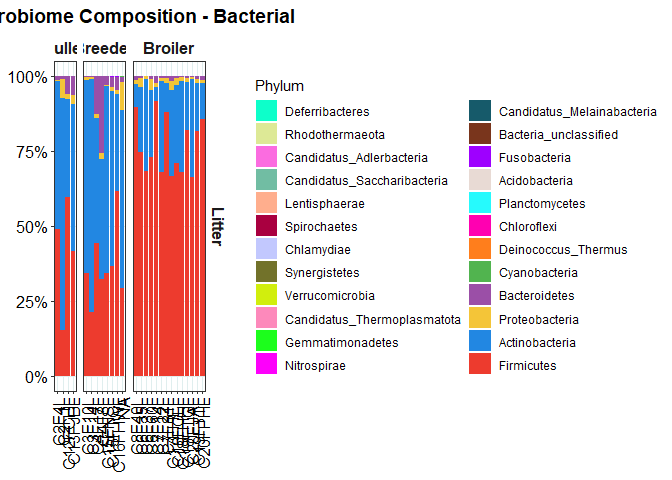
\includegraphics{Final_Project_Pankaj_files/figure-latex/drawing averaged relab plots-1.pdf}

\begin{Shaded}
\begin{Highlighting}[]
\NormalTok{relbp\_av\_bac\_Soil}
\end{Highlighting}
\end{Shaded}

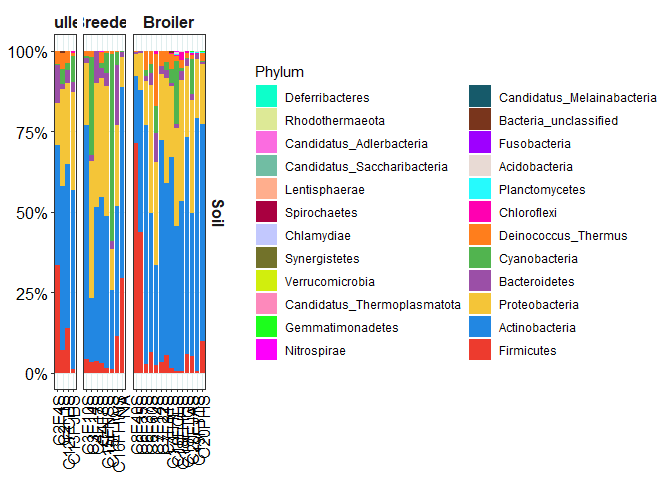
\includegraphics{Final_Project_Pankaj_files/figure-latex/drawing averaged relab plots-2.pdf}
Saving combined relative abundance plots

\begin{Shaded}
\begin{Highlighting}[]
\CommentTok{\#Saving plots}

\CommentTok{\#Combined plots}
\NormalTok{combined\_plot\_relative\_abundance\_bacteria }\OtherTok{\textless{}{-}} \FunctionTok{ggarrange}\NormalTok{(relbp\_av\_bac\_Litter, relbp\_av\_bac\_Soil,}
                           \AttributeTok{ncol =} \DecValTok{1}\NormalTok{,}
                           \AttributeTok{nrow =} \DecValTok{2}\NormalTok{,}
                           \AttributeTok{common.legend =} \ConstantTok{TRUE}\NormalTok{,}
                           \AttributeTok{legend =} \StringTok{"right"}\NormalTok{)}

\CommentTok{\#Saving plots}
\FunctionTok{ggsave}\NormalTok{(}\AttributeTok{filename =} \StringTok{"Relative\_abundance\_Plots.svg"}\NormalTok{,}
       \AttributeTok{plot =}\NormalTok{ combined\_plot\_relative\_abundance\_bacteria,}
       \AttributeTok{device =} \StringTok{"svg"}\NormalTok{,}
       \AttributeTok{units =} \StringTok{"mm"}\NormalTok{,}
       \AttributeTok{width =} \DecValTok{350}\NormalTok{,}
       \AttributeTok{height =} \DecValTok{220}\NormalTok{)}
\end{Highlighting}
\end{Shaded}

\section{\texorpdfstring{\textbf{Exploring
Beta-Diversity}}{Exploring Beta-Diversity}}\label{exploring-beta-diversity}

If alpha-diversity is the diversity \emph{within} a community,
beta-diversity is the diversity across communities. In beta-diversity we
are concerned with comparing and contrasting different profiles.

Communities can be statistically compared by producing distance
matrices. On compositional data we will use robust Aitchison distances,
which relies on the centered log ratio transform. Once these distances
are calculated, profiles can be statistically compared using PERMANOVA
and visualized using ordination plots, such as PCoA or PCA.

In order to perform these analysis the abundances will be again exported
into phyloseq but this time as relative abundances. The phyloseq object
will be used as input into two different packages: --\textgreater{}
Vegan: where PERMANOVA and PERMAdisp will be calculates --\textgreater{}
MicrobiomeMarker: where Ordinations and normalization will be performed

Creating relative abundance phyloseq object

\begin{Shaded}
\begin{Highlighting}[]
\NormalTok{OTUcount }\OtherTok{=} \FunctionTok{otu\_table}\NormalTok{(tbl\_otu, }
                \AttributeTok{taxa\_are\_rows =} \ConstantTok{TRUE}\NormalTok{)}
      \CommentTok{\#Needs to be parsed as matrix.}
\NormalTok{TAX }\OtherTok{=} \FunctionTok{tax\_table}\NormalTok{(}\FunctionTok{as.matrix}\NormalTok{(mt\_tax)}
\NormalTok{                )}
      \CommentTok{\#Needs to be parsed as matrix.}
\NormalTok{sampledata }\OtherTok{=} \FunctionTok{sample\_data}\NormalTok{(mt\_smpl)}

\CommentTok{\#Creating phyloseq objects}
\NormalTok{phycount }\OtherTok{=} \FunctionTok{phyloseq}\NormalTok{(OTUcount, TAX, sampledata)}


\CommentTok{\#Excluding Unclassified, Archaea and Dropping incomplete sample groups: Larvae and Pollen}
\NormalTok{phycount }\OtherTok{\textless{}{-}}\NormalTok{ phycount }\SpecialCharTok{\%\textgreater{}\%}
  \FunctionTok{subset\_taxa}\NormalTok{(}\SpecialCharTok{!}\NormalTok{Phylum }\SpecialCharTok{==} \StringTok{"UNCLASSIFIED"} \SpecialCharTok{\&} \SpecialCharTok{!}\NormalTok{Kingdom }\SpecialCharTok{==} \StringTok{"Archaea"} \SpecialCharTok{\&} \SpecialCharTok{!}\NormalTok{Kingdom }\SpecialCharTok{==} \StringTok{"Eukaryota"}\NormalTok{) }\SpecialCharTok{\%\textgreater{}\%}
  \FunctionTok{subset\_samples}\NormalTok{(}\SpecialCharTok{!}\NormalTok{Sample\_type }\SpecialCharTok{==} \StringTok{"Fecal"} \SpecialCharTok{\&} \SpecialCharTok{!}\NormalTok{Farm\_type }\SpecialCharTok{==} \StringTok{"Processing\_plant"}\NormalTok{)}
\end{Highlighting}
\end{Shaded}

\begin{Shaded}
\begin{Highlighting}[]
\CommentTok{\# printing phyloseq summary}

\NormalTok{phycount}
\end{Highlighting}
\end{Shaded}

\begin{verbatim}
## phyloseq-class experiment-level object
## otu_table()   OTU Table:         [ 3506 taxa and 62 samples ]
## sample_data() Sample Data:       [ 62 samples by 7 sample variables ]
## tax_table()   Taxonomy Table:    [ 3506 taxa by 7 taxonomic ranks ]
\end{verbatim}

\begin{Shaded}
\begin{Highlighting}[]
\FunctionTok{print}\NormalTok{(}\StringTok{""}\NormalTok{)}
\end{Highlighting}
\end{Shaded}

\begin{verbatim}
## [1] ""
\end{verbatim}

\begin{Shaded}
\begin{Highlighting}[]
\FunctionTok{print}\NormalTok{(}\StringTok{"Unique Phyla in phycount Object"}\NormalTok{)}
\end{Highlighting}
\end{Shaded}

\begin{verbatim}
## [1] "Unique Phyla in phycount Object"
\end{verbatim}

\begin{Shaded}
\begin{Highlighting}[]
\FunctionTok{get\_taxa\_unique}\NormalTok{(phycount, }\StringTok{"Phylum"}\NormalTok{)}
\end{Highlighting}
\end{Shaded}

\begin{verbatim}
##  [1] "Firmicutes"                  "Actinobacteria"             
##  [3] "Bacteroidetes"               "Proteobacteria"             
##  [5] "Cyanobacteria"               "Bacteria_unclassified"      
##  [7] "Deinococcus_Thermus"         "Acidobacteria"              
##  [9] "Planctomycetes"              "Chloroflexi"                
## [11] "Gemmatimonadetes"            "Nitrospirae"                
## [13] "Verrucomicrobia"             "Fusobacteria"               
## [15] "Candidatus_Melainabacteria"  "Lentisphaerae"              
## [17] "Synergistetes"               "Chlamydiae"                 
## [19] "Spirochaetes"                "Rhodothermaeota"            
## [21] "Deferribacteres"             "Candidatus_Adlerbacteria"   
## [23] "Candidatus_Saccharibacteria"
\end{verbatim}

\begin{Shaded}
\begin{Highlighting}[]
\FunctionTok{print}\NormalTok{(}\StringTok{"Sample Sources in phycount object"}\NormalTok{)}
\end{Highlighting}
\end{Shaded}

\begin{verbatim}
## [1] "Sample Sources in phycount object"
\end{verbatim}

\begin{Shaded}
\begin{Highlighting}[]
\FunctionTok{levels}\NormalTok{(}\FunctionTok{sample\_data}\NormalTok{(phycount)}\SpecialCharTok{$}\NormalTok{Sample\_type)}
\end{Highlighting}
\end{Shaded}

\begin{verbatim}
## [1] "Litter" "Soil"
\end{verbatim}

\begin{Shaded}
\begin{Highlighting}[]
\FunctionTok{levels}\NormalTok{(}\FunctionTok{sample\_data}\NormalTok{(phycount)}\SpecialCharTok{$}\NormalTok{Farm\_type)}
\end{Highlighting}
\end{Shaded}

\begin{verbatim}
## [1] "Pullet"  "Breeder" "Broiler"
\end{verbatim}

\#\#Performing PERMANOVAS

\begin{itemize}
\tightlist
\item
  PERMANOVA, (permutational multivariate ANOVA), is a non-parametric
  alternative to MANOVA, or multivariate ANOVA test.
\item
  PERMANOVAS are calculated using the adonis functions in the package
  Vegan. To use Vegan, phyloseq objects need to be turned into Vegan
  objects.
\item
  Next functions convert physeq format into Vegan.
\end{itemize}

creating pssd2veg function

\begin{Shaded}
\begin{Highlighting}[]
\NormalTok{pssd2veg }\OtherTok{\textless{}{-}} \ControlFlowTok{function}\NormalTok{(physeq) \{}
\NormalTok{  sd }\OtherTok{\textless{}{-}} \FunctionTok{sample\_data}\NormalTok{(physeq)}
  \FunctionTok{return}\NormalTok{(}\FunctionTok{as}\NormalTok{(sd,}\StringTok{"data.frame"}\NormalTok{))}
\NormalTok{\}}
\end{Highlighting}
\end{Shaded}

Creating psotu2veg function

\begin{Shaded}
\begin{Highlighting}[]
\NormalTok{psotu2veg }\OtherTok{\textless{}{-}} \ControlFlowTok{function}\NormalTok{(physeq) \{}
\NormalTok{  OTU }\OtherTok{\textless{}{-}} \FunctionTok{otu\_table}\NormalTok{(physeq)}
  \ControlFlowTok{if}\NormalTok{ (}\FunctionTok{taxa\_are\_rows}\NormalTok{(OTU)) \{}
\NormalTok{    OTU }\OtherTok{\textless{}{-}} \FunctionTok{t}\NormalTok{(OTU)}
\NormalTok{  \}}
  \FunctionTok{return}\NormalTok{(}\FunctionTok{as}\NormalTok{(OTU, }\StringTok{"matrix"}\NormalTok{))}
\NormalTok{\}}
\end{Highlighting}
\end{Shaded}

Importing Phyloseq data into teh package Vegan

\begin{Shaded}
\begin{Highlighting}[]
\NormalTok{vegan\_count }\OtherTok{\textless{}{-}} \FunctionTok{pssd2veg}\NormalTok{(phycount)}
\NormalTok{vegan\_otu }\OtherTok{\textless{}{-}} \FunctionTok{psotu2veg}\NormalTok{(phycount)}
\end{Highlighting}
\end{Shaded}

Calculating distance matrix

\begin{Shaded}
\begin{Highlighting}[]
\DocumentationTok{\#\#Calculating distance matrix using Robust Aitchinson (Euclidean distance of the CLR transform of non{-}zero values)}
\NormalTok{veg\_count\_raitch }\OtherTok{\textless{}{-}} \FunctionTok{vegdist}\NormalTok{(vegan\_otu, }\StringTok{"robust.aitchison"}\NormalTok{)}
\end{Highlighting}
\end{Shaded}

\subsection{RUNNING PERMANOVAs}\label{running-permanovas}

\begin{Shaded}
\begin{Highlighting}[]
\CommentTok{\#Writing the overall PERMANOVA results in text file}
\FunctionTok{sink}\NormalTok{(}\StringTok{"PERMANOVA\_Overall\_Results.txt"}\NormalTok{)}


\FunctionTok{set.seed}\NormalTok{(}\DecValTok{43}\NormalTok{)}

\FunctionTok{print}\NormalTok{(}\StringTok{"Comparing profiles by PERMANOVA"}\NormalTok{,}\AttributeTok{quote =} \ConstantTok{FALSE}\NormalTok{, }\AttributeTok{justify =} \StringTok{"centre"}\NormalTok{)}
\FunctionTok{print}\NormalTok{(}\StringTok{"Grouping by Sample\_group (Sample\_type*Farm\_type*Company"}\NormalTok{,}\AttributeTok{quote =} \ConstantTok{FALSE}\NormalTok{, }\AttributeTok{justify =} \StringTok{"centre"}\NormalTok{)}

\FunctionTok{adonis2}\NormalTok{(veg\_count\_raitch }\SpecialCharTok{\textasciitilde{}}\NormalTok{ Sample\_type}\SpecialCharTok{*}\NormalTok{Farm\_type}\SpecialCharTok{*}\NormalTok{Company, }\AttributeTok{data =}\NormalTok{ vegan\_count, }\AttributeTok{permutations =} \DecValTok{999}\NormalTok{)}
\FunctionTok{print}\NormalTok{(}\StringTok{""}\NormalTok{,}\AttributeTok{quote =} \ConstantTok{FALSE}\NormalTok{, }\AttributeTok{justify =} \StringTok{"centre"}\NormalTok{)}
\FunctionTok{print}\NormalTok{(}\StringTok{"Grouping by Sample\_type"}\NormalTok{,}\AttributeTok{quote =} \ConstantTok{FALSE}\NormalTok{, }\AttributeTok{justify =} \StringTok{"centre"}\NormalTok{)}

\FunctionTok{adonis2}\NormalTok{(veg\_count\_raitch }\SpecialCharTok{\textasciitilde{}}\NormalTok{ Sample\_type, }\AttributeTok{data =}\NormalTok{ vegan\_count, }\AttributeTok{permutations =} \DecValTok{999}\NormalTok{)}
\FunctionTok{print}\NormalTok{(}\StringTok{""}\NormalTok{,}\AttributeTok{quote =} \ConstantTok{FALSE}\NormalTok{, }\AttributeTok{justify =} \StringTok{"centre"}\NormalTok{)}
\FunctionTok{print}\NormalTok{(}\StringTok{"Grouping by Farm\_type"}\NormalTok{,}\AttributeTok{quote =} \ConstantTok{FALSE}\NormalTok{, }\AttributeTok{justify =} \StringTok{"centre"}\NormalTok{)}

\FunctionTok{adonis2}\NormalTok{(veg\_count\_raitch }\SpecialCharTok{\textasciitilde{}}\NormalTok{ Farm\_type, }\AttributeTok{data =}\NormalTok{ vegan\_count, }\AttributeTok{permutations =} \DecValTok{999}\NormalTok{)}
\FunctionTok{print}\NormalTok{(}\StringTok{""}\NormalTok{,}\AttributeTok{quote =} \ConstantTok{FALSE}\NormalTok{, }\AttributeTok{justify =} \StringTok{"centre"}\NormalTok{)}
\FunctionTok{print}\NormalTok{(}\StringTok{"Grouping by Company"}\NormalTok{,}\AttributeTok{quote =} \ConstantTok{FALSE}\NormalTok{, }\AttributeTok{justify =} \StringTok{"centre"}\NormalTok{)}

\FunctionTok{adonis2}\NormalTok{(veg\_count\_raitch }\SpecialCharTok{\textasciitilde{}}\NormalTok{ Company, }\AttributeTok{data =}\NormalTok{ vegan\_count, }\AttributeTok{permutations =} \DecValTok{999}\NormalTok{)}

\FunctionTok{sink}\NormalTok{()}
\end{Highlighting}
\end{Shaded}

Specific adonis pariwise comparision

\begin{Shaded}
\begin{Highlighting}[]
\CommentTok{\#Writing the specific pariwise comparission of interest in text file}
\FunctionTok{sink}\NormalTok{(}\StringTok{"specific\_Pairwise\_Comparissions\_PERMANOVA.txt"}\NormalTok{)}

\DocumentationTok{\#\# Install pairwiseAdonis package if not already installed}
\CommentTok{\#if (!requireNamespace("devtools", quietly = TRUE)) \{}
\CommentTok{\# install.packages("devtools")}
\CommentTok{\#\}}
\CommentTok{\#devtools::install\_github("pmartinezarbizu/pairwiseAdonis/pairwiseAdonis")}

\CommentTok{\# Load the package}
\FunctionTok{library}\NormalTok{(pairwiseAdonis)}
\end{Highlighting}
\end{Shaded}

\begin{verbatim}
## Loading required package: cluster
\end{verbatim}

\begin{Shaded}
\begin{Highlighting}[]
\CommentTok{\# Perform pairwise PERMANOVA for Sample\_type}
\FunctionTok{pairwise.adonis2}\NormalTok{(veg\_count\_raitch }\SpecialCharTok{\textasciitilde{}}\NormalTok{ Sample\_type, }\AttributeTok{data =}\NormalTok{ vegan\_count, }\AttributeTok{permutations =} \DecValTok{999}\NormalTok{)}

\CommentTok{\# Perform pairwise PERMANOVA for Farm\_type}
\FunctionTok{pairwise.adonis2}\NormalTok{(veg\_count\_raitch }\SpecialCharTok{\textasciitilde{}}\NormalTok{ Farm\_type, }\AttributeTok{data =}\NormalTok{ vegan\_count, }\AttributeTok{permutations =} \DecValTok{999}\NormalTok{)}


\FunctionTok{sink}\NormalTok{()}
\end{Highlighting}
\end{Shaded}

\subsubsection{ORDINATION WITH PCOA}\label{ordination-with-pcoa}

Drawing PCA plots

\begin{Shaded}
\begin{Highlighting}[]
\CommentTok{\#Sample type}
\NormalTok{pcoa\_sp\_clr\_S }\OtherTok{\textless{}{-}}
\NormalTok{  phycount }\SpecialCharTok{\%\textgreater{}\%}
 \FunctionTok{tax\_transform}\NormalTok{(}\AttributeTok{rank =} \StringTok{"Species"}\NormalTok{, }
               \AttributeTok{trans =} \StringTok{"identity"}\NormalTok{) }\SpecialCharTok{\%\textgreater{}\%}  
 \FunctionTok{dist\_calc}\NormalTok{(}\AttributeTok{dist =} \StringTok{"robust.aitchison"}\NormalTok{) }\SpecialCharTok{\%\textgreater{}\%}
 \FunctionTok{ord\_calc}\NormalTok{(}\AttributeTok{method =} \StringTok{"PCoA"}\NormalTok{) }\SpecialCharTok{\%\textgreater{}\%} 
 \FunctionTok{ord\_plot}\NormalTok{(}\AttributeTok{axes =} \FunctionTok{c}\NormalTok{(}\DecValTok{1}\NormalTok{, }\DecValTok{2}\NormalTok{),}
          \AttributeTok{plot\_taxa =} \DecValTok{1}\SpecialCharTok{:}\DecValTok{3}\NormalTok{,}
          \AttributeTok{colour =} \StringTok{"black"}\NormalTok{, }
          \AttributeTok{fill =} \StringTok{"Sample\_type"}\NormalTok{,}
          \AttributeTok{shape =} \StringTok{"Farm\_type"}\NormalTok{,}
          \AttributeTok{alpha =} \FloatTok{0.8}\NormalTok{,}
          \AttributeTok{size =} \DecValTok{5}
\NormalTok{          ) }\SpecialCharTok{+} 
  \FunctionTok{stat\_ellipse}\NormalTok{(}\FunctionTok{aes}\NormalTok{(}\AttributeTok{colour =}\NormalTok{ Sample\_type), }\AttributeTok{linewidth =} \FloatTok{0.3}\NormalTok{) }\SpecialCharTok{+}
  \FunctionTok{scale\_shape\_girafe\_filled}\NormalTok{() }\SpecialCharTok{+}
  \FunctionTok{ggtitle}\NormalTok{(}\StringTok{"PCoA Plot: Beta Diversity {-} Sample Types"}\NormalTok{) }\SpecialCharTok{+}
   \FunctionTok{guides}\NormalTok{(}\AttributeTok{fill =} \FunctionTok{guide\_legend}\NormalTok{(}\AttributeTok{override.aes=}\FunctionTok{list}\NormalTok{(}\AttributeTok{shape =} \DecValTok{21}\NormalTok{)),}
          \AttributeTok{color =} \ConstantTok{FALSE}\NormalTok{) }\SpecialCharTok{+}
  \FunctionTok{scale\_fill\_manual}\NormalTok{(}\AttributeTok{values =}\NormalTok{ col\_sample) }\SpecialCharTok{+}
  \CommentTok{\# scale\_color\_manual(values = col\_sample) +}
  \CommentTok{\# scale\_alpha\_discrete(range = c(0.35, 1)) +}
  \FunctionTok{theme\_linedraw}\NormalTok{() }\SpecialCharTok{+}
  \FunctionTok{theme}\NormalTok{(}\AttributeTok{panel.grid =} \FunctionTok{element\_blank}\NormalTok{(),}
        \AttributeTok{panel.background =} \FunctionTok{element\_rect}\NormalTok{(}\AttributeTok{fill =} \StringTok{"\#fdfdfd"}\NormalTok{),}
        \AttributeTok{axis.text =} \FunctionTok{element\_text}\NormalTok{(}\AttributeTok{size =} \DecValTok{14}\NormalTok{,}
                                 \AttributeTok{color =} \StringTok{"black"}\NormalTok{),}
        \AttributeTok{axis.title =} \FunctionTok{element\_text}\NormalTok{(}\AttributeTok{size =} \DecValTok{16}\NormalTok{,}
                                  \AttributeTok{color =} \StringTok{"black"}\NormalTok{)) }\SpecialCharTok{+}
  \FunctionTok{geom\_text}\NormalTok{(}\AttributeTok{x =} \FloatTok{2.5}\NormalTok{, }
            \AttributeTok{y =} \SpecialCharTok{{-}}\FloatTok{3.4}\NormalTok{, }
            \AttributeTok{hjust =}\DecValTok{0}\NormalTok{,}
            \AttributeTok{vjust =} \DecValTok{1}\NormalTok{,}
            \AttributeTok{label=}\StringTok{"Sample Type:}\SpecialCharTok{\textbackslash{}n}\StringTok{PERMANOVA=0.001"}\NormalTok{,}
            \AttributeTok{size =} \FloatTok{3.5}\NormalTok{,}
            \AttributeTok{fontface =} \StringTok{"plain"}\NormalTok{)}
\end{Highlighting}
\end{Shaded}

\begin{verbatim}
## Warning: otu_table of counts is NOT available!
## Available otu_table contains 16736 values that are not non-negative integers
\end{verbatim}

\begin{verbatim}
## Warning: The `<scale>` argument of `guides()` cannot be `FALSE`. Use "none" instead as
## of ggplot2 3.3.4.
## This warning is displayed once every 8 hours.
## Call `lifecycle::last_lifecycle_warnings()` to see where this warning was
## generated.
\end{verbatim}

\begin{Shaded}
\begin{Highlighting}[]
\CommentTok{\#Farm type}
\NormalTok{pcoa\_sp\_clr\_farm }\OtherTok{\textless{}{-}}
\NormalTok{  phycount }\SpecialCharTok{\%\textgreater{}\%}
 \FunctionTok{tax\_transform}\NormalTok{(}\AttributeTok{rank =} \StringTok{"Species"}\NormalTok{, }
               \AttributeTok{trans =} \StringTok{"identity"}\NormalTok{) }\SpecialCharTok{\%\textgreater{}\%}  
 \FunctionTok{dist\_calc}\NormalTok{(}\AttributeTok{dist =} \StringTok{"robust.aitchison"}\NormalTok{) }\SpecialCharTok{\%\textgreater{}\%}
 \FunctionTok{ord\_calc}\NormalTok{(}\AttributeTok{method =} \StringTok{"PCoA"}\NormalTok{) }\SpecialCharTok{\%\textgreater{}\%} 
 \FunctionTok{ord\_plot}\NormalTok{(}\AttributeTok{axes =} \FunctionTok{c}\NormalTok{(}\DecValTok{1}\NormalTok{, }\DecValTok{2}\NormalTok{),}
          \AttributeTok{plot\_taxa =} \DecValTok{1}\SpecialCharTok{:}\DecValTok{3}\NormalTok{,}
          \AttributeTok{colour =} \StringTok{"black"}\NormalTok{, }
          \AttributeTok{fill =} \StringTok{"Farm\_type"}\NormalTok{,}
          \AttributeTok{shape =} \StringTok{"Sample\_type"}\NormalTok{,}
          \AttributeTok{alpha =} \FloatTok{0.8}\NormalTok{,}
          \AttributeTok{size =} \DecValTok{5}
\NormalTok{          ) }\SpecialCharTok{+} 
  \FunctionTok{stat\_ellipse}\NormalTok{(}\FunctionTok{aes}\NormalTok{(}\AttributeTok{colour =}\NormalTok{ Farm\_type), }\AttributeTok{linewidth =} \FloatTok{0.3}\NormalTok{) }\SpecialCharTok{+}
  \FunctionTok{scale\_shape\_girafe\_filled}\NormalTok{() }\SpecialCharTok{+}
  \FunctionTok{ggtitle}\NormalTok{(}\StringTok{"PCoA Plot: Beta Diversity {-} Farm Types"}\NormalTok{) }\SpecialCharTok{+}
   \FunctionTok{guides}\NormalTok{(}\AttributeTok{fill =} \FunctionTok{guide\_legend}\NormalTok{(}\AttributeTok{override.aes=}\FunctionTok{list}\NormalTok{(}\AttributeTok{shape =} \DecValTok{21}\NormalTok{)),}
          \AttributeTok{color =} \ConstantTok{FALSE}\NormalTok{) }\SpecialCharTok{+}
  \FunctionTok{scale\_fill\_manual}\NormalTok{(}\AttributeTok{values =}\NormalTok{ col\_farm) }\SpecialCharTok{+}
  \FunctionTok{scale\_color\_manual}\NormalTok{(}\AttributeTok{values =}\NormalTok{ col\_farm) }\SpecialCharTok{+}
  \CommentTok{\# scale\_alpha\_discrete(range = c(0.35, 1)) +}
  \FunctionTok{theme\_linedraw}\NormalTok{() }\SpecialCharTok{+}
  \FunctionTok{theme}\NormalTok{(}\AttributeTok{panel.grid =} \FunctionTok{element\_blank}\NormalTok{(),}
        \AttributeTok{panel.background =} \FunctionTok{element\_rect}\NormalTok{(}\AttributeTok{fill =} \StringTok{"\#fdfdfd"}\NormalTok{),}
        \AttributeTok{axis.text =} \FunctionTok{element\_text}\NormalTok{(}\AttributeTok{size =} \DecValTok{14}\NormalTok{,}
                                 \AttributeTok{color =} \StringTok{"black"}\NormalTok{),}
        \AttributeTok{axis.title =} \FunctionTok{element\_text}\NormalTok{(}\AttributeTok{size =} \DecValTok{16}\NormalTok{,}
                                  \AttributeTok{color =} \StringTok{"black"}\NormalTok{)) }\SpecialCharTok{+}
  \FunctionTok{geom\_text}\NormalTok{(}\AttributeTok{x =} \FloatTok{2.5}\NormalTok{, }
            \AttributeTok{y =} \SpecialCharTok{{-}}\FloatTok{3.4}\NormalTok{, }
            \AttributeTok{hjust =}\DecValTok{0}\NormalTok{,}
            \AttributeTok{vjust =} \DecValTok{1}\NormalTok{,}
            \AttributeTok{label=}\StringTok{"Farm Type:}\SpecialCharTok{\textbackslash{}n}\StringTok{PERMANOVA=0.001"}\NormalTok{,}
            \AttributeTok{size =} \FloatTok{3.5}\NormalTok{,}
            \AttributeTok{fontface =} \StringTok{"plain"}\NormalTok{) }\CommentTok{\#+}
\end{Highlighting}
\end{Shaded}

\begin{verbatim}
## Warning: otu_table of counts is NOT available!
## Available otu_table contains 16736 values that are not non-negative integers
\end{verbatim}

\begin{Shaded}
\begin{Highlighting}[]
  \CommentTok{\#facet\_grid(. \textasciitilde{} Company, scale = "free")}
\end{Highlighting}
\end{Shaded}

\begin{Shaded}
\begin{Highlighting}[]
\NormalTok{pcoa\_sp\_clr\_S}
\end{Highlighting}
\end{Shaded}

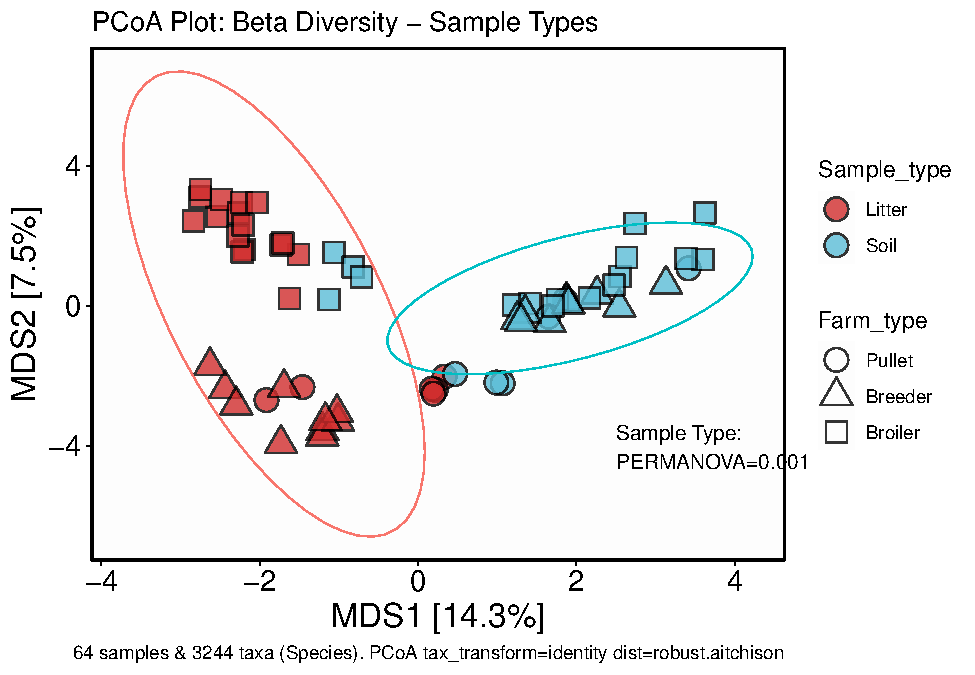
\includegraphics{Final_Project_Pankaj_files/figure-latex/drawing PCoA plots-1.pdf}

\begin{Shaded}
\begin{Highlighting}[]
\NormalTok{pcoa\_sp\_clr\_farm}
\end{Highlighting}
\end{Shaded}

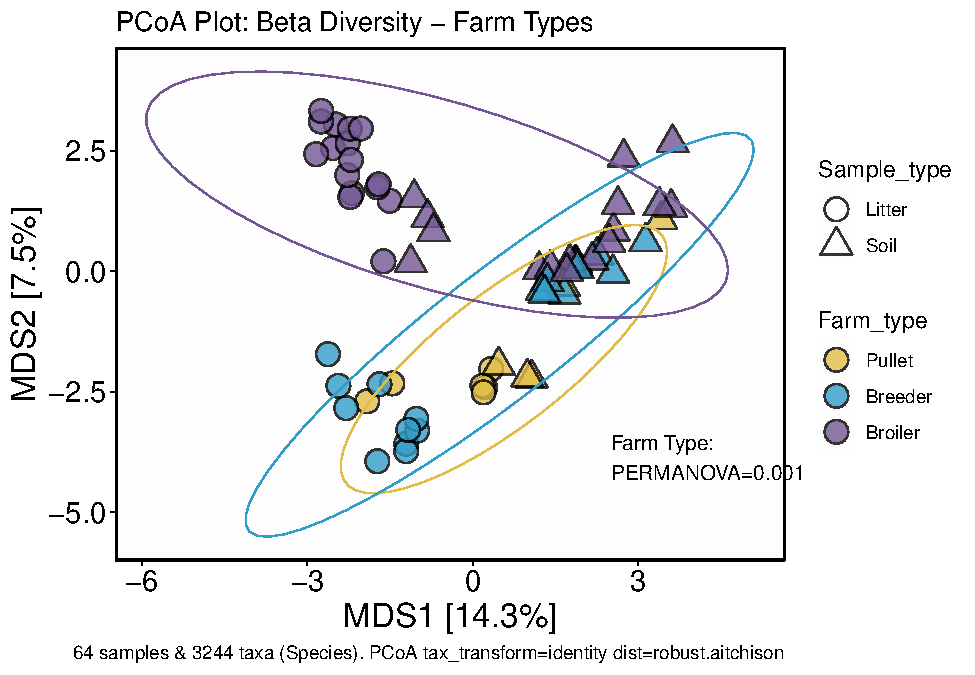
\includegraphics{Final_Project_Pankaj_files/figure-latex/drawing PCoA plots-2.pdf}
Saving combined beta diversity - PCoA plots

\begin{Shaded}
\begin{Highlighting}[]
\CommentTok{\#Combined plots}
\NormalTok{combined\_PCoA }\OtherTok{\textless{}{-}} \FunctionTok{ggarrange}\NormalTok{(pcoa\_sp\_clr\_S, pcoa\_sp\_clr\_farm,}
                           \AttributeTok{ncol =} \DecValTok{1}\NormalTok{,}
                           \AttributeTok{nrow =} \DecValTok{2}\NormalTok{)}


\FunctionTok{ggsave}\NormalTok{(}\AttributeTok{filename =} \StringTok{"Combined\_PCoA\_plots\_betadiversity.svg"}\NormalTok{,}
        \AttributeTok{plot =}\NormalTok{ combined\_PCoA,}
        \AttributeTok{device =} \StringTok{"svg"}\NormalTok{,}
        \AttributeTok{units =} \StringTok{"mm"}\NormalTok{,}
        \AttributeTok{width =} \DecValTok{250}\NormalTok{,}
        \AttributeTok{height =} \DecValTok{300}\NormalTok{)}
\end{Highlighting}
\end{Shaded}

\section{Link to GitHub repository}\label{link-to-github-repository}

\href{https://github.com/ppg0001/PLPA_Assignment}{Click here to go to
GitHub repository}

\end{document}
